\documentclass[a4paper,12pt, openany]{book}


%%% Работа с русским языком
\usepackage{cmap}          % поиск в PDF
\usepackage[T2A]{fontenc}      % кодировка
\usepackage[utf8]{inputenc}    % кодировка исходного текста
%\usepackage{fixint}
\usepackage[russian]{babel}  % локализация и переносы
%\usepackage{pscyr}
\usepackage{mathtools, nccmath}
%\renewcommand{\rmdefault}{cmss}
%%% Дополнительная работа с математикой
\usepackage{amsmath,amsfonts,amssymb,amsthm,mathtools} % AMS
\usepackage{titlesec}
\titleformat{\section}{\filcenter\rmfamily\Large\bfseries}{\thesection.}{0.2em}{}
\titleformat{\subsection}{\filcenter\rmfamily\large\bfseries}{\thesubsection.}{0.2em}{}
\titleformat{\subsubsection}{\filcenter\rmfamily\large\bfseries}{\thesubsubsection.}{0.2em}{}
%% Номера формул
%\mathtoolsset{showonlyrefs=true} % Показывать номера только у тех формул, на которые есть \eqref{} в тексте.
%\usepackage{leqno} % Нумерация формул слева
%\usepackage{rumathgrk1}
%\usepackage{MnSymbol}
%% Перенос знаков в формулах (по Львовскому)
\newcommand{\hm}[1]{#1\nobreak\discretionary{}{\hbox{\ensuremath{#1}}}{}}
%\usepackage{glonti}
%%% Работа с картинками
\usepackage{graphicx}  % Для вставки рисунков

\graphicspath{{images/}}  % папки с картинками
\usepackage{wrapfig} % Обтекание рисунков текстом
\addto\captionsrussian{\def\refname{Список используемой литературы}}
%%% Работа с таблицами
\usepackage{array,tabularx,tabulary} % Дополнительная работа с таблицами
\usepackage{longtable}  % Длинные таблицы
\usepackage{multirow} % Слияние строк в таблице
%%% Теоремы
\theoremstyle{plain} % Это стиль по умолчанию, его можно не переопределять.
\newtheorem{theorem}{Теорема}[section]
\newtheorem{proposition}[theorem]{Утверждение}
\usepackage{subcaption}
\theoremstyle{definition} % "Определение"
\newtheorem{corollary}{Следствие}[theorem]
\newtheorem{problem}{Задача}[section]
\pagestyle{plain}
\theoremstyle{remark} % "Примечание"
\newtheorem*{nonum}{Решение}
%\pagestyle{empty}
%%% Страница
\usepackage{extsizes} % Возможность сделать 14-й шрифт
\usepackage{geometry} % Простой способ задавать поля
\geometry{top=20mm}
%\geometry{bottom=35mm}
\geometry{left=20mm}
\geometry{right=20mm}
\setlength{\parindent}{1.1cm}
%\numberwithin{equation}{section}
\usepackage{setspace} % Интерлиньяж
%\onehalfspacing % Интерлиньяж 1.5
%\doublespacing % Интерлиньяж 2
%\singlespacing % Интерлиньяж 1
\makeatletter
\def\@biblabel#1{#1. }
\makeatother
\usepackage{misccorr}
\usepackage{lastpage} % Узнать, сколько всего страниц в документе.
\usepackage[usenames]{color}
\usepackage{colortbl}
\renewcommand{\baselinestretch}{1.07}
\usepackage{hyperref}

\usepackage[usenames,dvipsnames,svgnames,table]{xcolor}
\hypersetup{        % Гиперссылки
  unicode=true,           % русские буквы в раздела PDF
  pdftitle={Заголовок},   % Заголовок
  pdfauthor={Автор},      % Автор
  pdfsubject={Тема},      % Тема
  pdfcreator={Создатель}, % Создатель
  pdfproducer={Производитель}, % Производитель
  pdfkeywords={keyword1} {key2} {key3}, % Ключевые слова
  colorlinks=true,         % false: ссылки в рамках; true: цветные ссылки
  linkcolor=black,          % внутренние ссылки
  citecolor=blue,        % на библиографию
  filecolor=magenta,      % на файлы
  urlcolor=cyan           % на URL
}
\usepackage{bm}
\usepackage{todonotes}
\usepackage{booktabs}
\newcommand{\dd}{\mathrm{d}}
\numberwithin{equation}{chapter}

\begin{document}
\listoftodos
\newpage
\thispagestyle{empty}


% НАЧАЛО ТИТУЛЬНОГО ЛИСТА
\begin{center}
    \large{\textsc{ФЕДЕРАЛЬНОЕ ГОСУДАРСТВЕННОЕ БЮДЖЕТНОЕ ОБРАЗОВАТЕЛЬНОЕ
            УЧРЕЖДЕНИЕ ВЫСШЕГО ОБРАЗОВАНИЯ}
    }\\
    \large{\textsc{МОСКОВСКИЙ ГОСУДАРСТВЕННЫЙ УНИВЕРСИТЕТ имени М.В. ЛОМОНОСОВА}
    } \\
    \vspace{0.4cm}
    \large{\textsc{МЕХАНИКО - МАТЕМАТИЧЕСКИЙ ФАКУЛЬТЕТ}}\\
    \vspace{0.4cm}
    \large{\textsc{КАФЕДРА ПРИКЛАДНОЙ МЕХАНИКИ И УПРАВЛЕНИЯ}}\\
    \hfill \break

    \hfill \break
    \large{\textbf{ВЫПУСКНАЯ КВАЛИФИКАЦИОННАЯ РАБОТА}\\
        (ДИПЛОМНАЯ РАБОТА) \\ МАГИСТРА \\
        \hfill \break \textsc{\textbf{ВОССТАНОВЛЕНИЕ ЧЕЛОВЕКОМ ИСХОДНОЙ ПОЗЫ ПОСЛЕ ТОЛЧКА}
        }}
\end{center}

\vspace{1.5cm}
\begin{flushright}
    \large{
        Выполнил: студент группы М - 2 \\ Романов Андрей Владимирович} \\ \vspace{0.68cm}  \underline{\hspace{6.5cm}} \\
    (подпись студента)

\end{flushright}

\begin{flushright}
    \large{
        Научный руководитель: \\ к.ф.-м.н., доцент Кручинин Павел Анатольевич} \\ \vspace{0.68cm}
    \underline{\hspace{6.5cm}} \\
    (подпись научного руководителя)
\end{flushright}
\vspace{0.7cm}
\begin{center} \large{Москва \\  2023} \end{center}



\thispagestyle{empty} % выключаем отображение номера для этой страницы
\normalsize{
% КОНЕЦ ТИТУЛЬНОГО ЛИСТА
\newpage

\tableofcontents

\newpage

\addcontentsline{toc}{chapter}{Введение}

\chapter*{Введение}
В литературе встречается решение задач оптимального быстродействия для моделей движения человека \cite{pandy,humanMovements}. Исследование таких задач может помочь объяснить некоторые особенности результатов, наблюдаемых при обследованиях.
Проба со ступенчатым воздействием является одной из стандартных проб
при стабилометрических исследованиях \cite{AdaptFizkult,stabilographTest}. При проведении этой пробы
обследуемый стоит на платформе стабилоанализатора перед экраном, на
котором изображена мишень и отображается движение центра давления
человека, после толчка в спину, определяемое по показаниям стабилоанализатора.

В ходе теста производят толкающее воздействие на человека с помощью груза, помещенного на подвижном отвесе \cite{pusher}. В результате внешнего
воздействия тело человека наклоняется вперед и при не очень сильном толчке
он не теряет равновесие и не падает, а возвращается в исходное
положение за счет изменения угла в голеностопном суставе. Изменение
остальных суставных углов может оказаться тоже не столь значительным.
Родственные задачи уже решались в работах \cite{PAKrychinin,kasatkin}.
Схематическое изображение эксперимента представлено на рисунке \ref{fig:pusher}.
\begin{figure}[h!]
    \centering
    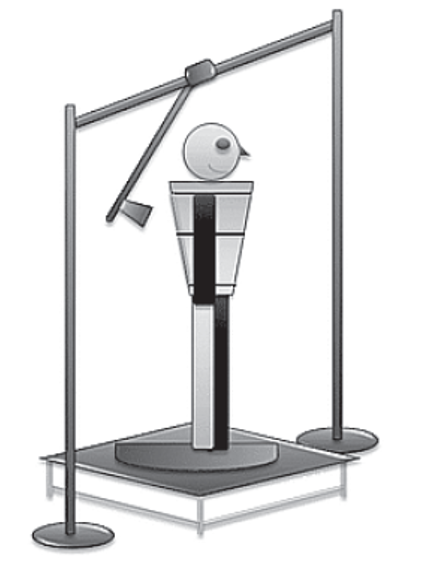
\includegraphics[width=0.35\linewidth]{human.png}
    \caption{Cхематическое изображение толкателя и
        положения испытуемого на стабилоплатформе}
    \label{fig:pusher}
\end{figure}

Исходные данные об отклонении сагиттальной коордианты при различных по силе толчках, предоставлены сотрудниками ИМБП РАН (см. рисунок \ref{fig:pushes})
\begin{figure}[h!]
    \centering
    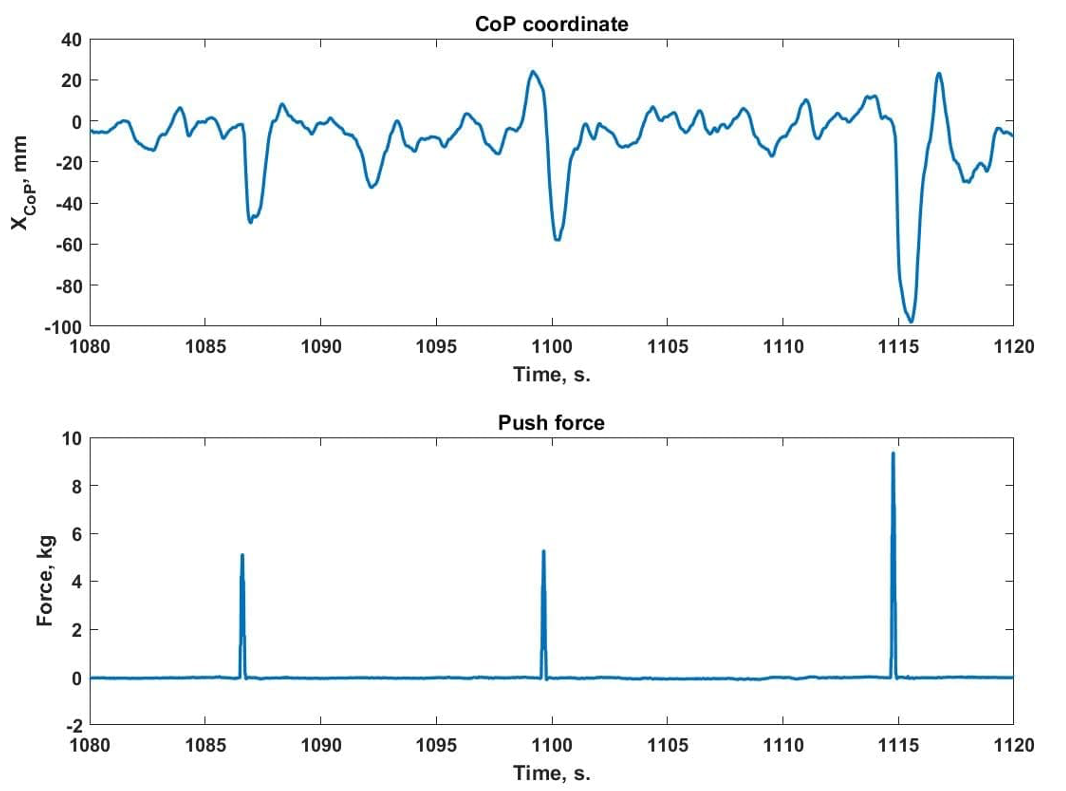
\includegraphics[width=0.9\linewidth]{Pushes.png}
    \caption{Отклонение сагиттальной координаты при различных по силе толчках}
    \label{fig:pushes}
\end{figure}
\todo[inline]{Картинку перерисовать с акутальными данными}
В качестве математической модели
используется традиционно модель «перевернутого маятника»\cite{PAKrychinin,kasatkin,gurfincel}.


\textbf{Целью работы} является разработка алгоритма управления изменением позы человека, основанного на решении задачи оптимального быстродействия,
который можно было бы использовать для возвращения в исходную вертикальную позу. В дальнейшем
такое решение предполагается использовать для оценки эффективности управления человеком
при возвращении в вертикальную позу, путем сравнения
времени реального процесса с полученным эталонным решением оптимальной задачи.

\textbf{Акутальность работы} объясняется тем, что похожие задачи уже решались, но именно эта с такими начальными условиям новая.
Решение это задачи может быть применено как в медицине, для оценки оптимальности работы мышщ человека, так и при разработке протезов, иммитирующих работу мышщ.

\textbf{Задачи работы: }
\begin{itemize}
    \item Описание математической модели
    \item Постановка задачи быстродействия, используя принцип максимума Понтрягина
    \item Поиск решения задачи быстродействия
    \item Определение начального состояния системы, в момент завершения толчка
    \item Решение задачи быстродействия с вычисленными начальными условиям
    \item Сравнение реального и оптимального времени возвращения в исходную позу
    \item Сравнение реальной и оптимальной траектории возварщения в исходную позу
    \item Интерпретация полученных результатов
\end{itemize}

\textbf{Методы исследования:}
\begin{itemize}
    \item Движение человека в саггительной плоскости описывается моделью перевернутого маятника.
    \item Для описание движения используется система обыкновенных дифференциальных уравнений с постоянными коэффицентами 3 порядка.
    \item Начальные условия для задачи быстродействия определяются с данных эксперимента, в ходе которого на человека оказывают толкающее воздействие.
    \item Проводится графическое моделирование в математических пакетах Matlab и Wolfram Mathematica.
\end{itemize}




\textbf{Объем и структура работы.} Работа состоит из введения, трех глав и заключения. Полный объем работы составляет 61 страницу, включая 69 рисунков и 1 таблицу. Список литературы содержит 17 наименований.

\newpage

\chapter{Математическая модель и решение задачи быстродействия}
\section{Математическая модель}
Для описания движения тела человека в сагиттальной плоскости используем традиционную модель перевернутого маятника (см. рисунок \ref{fig:pendulum}).

\begin{figure}[h!]
    \centering
    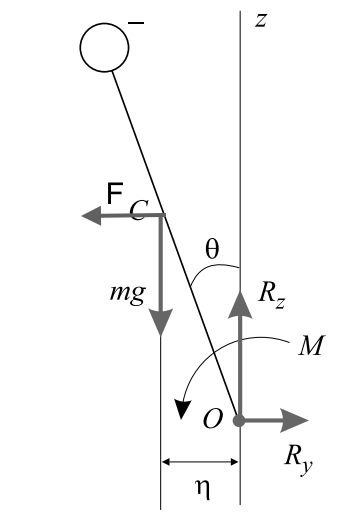
\includegraphics[width=0.4\linewidth]{body_1.png}
    \caption{Модель перевернутого маятника}
    \label{fig:pendulum}
\end{figure}

Традиционно предполагаем, что тело человека в ходе теста допустимо
моделировать недеформируемым однородным стержнем массы $m_T$,
закрепленным шарнирно в точке $O$, которая соответствует
голеностопному суставу.

Центр масс стержня расположен в точке $C$, удаленной от точки $O$
на расстояние $l$. Момент инерции стержня относительно фронтальной
оси, проходящей через точку $O$, равен $J$. Отклонение стержня от
вертикали описывается углом $\varphi$. Будем считать, что обследуемый
ориентирован так, что его сагиттальная плоскость параллельна оси
чувствительности платформы, а его стопа неподвижна относительно
платформы. Скорость изменения момента $M$, который приложен в точке $O$ к стержню,
будем считать управлением.

На тело воздействует два момента: первый от силы тяжести, второй момент возникает в голеностопе.
Запишем уравнение моментов,относительно точки $O$ на ось перпендикулярную плоскости рисунка \ref{fig:pendulum}
\[
    J\ddot{\varphi}= m_Tgl\sin\varphi+M
\]

Уравнение моментов для малых значений угла $\varphi$ и
скорости его изменения запишем, как традиционно принято для этой задачи.
\[
    J\ddot{\varphi}= m_Tgl\varphi+M
\]

Необходимо перевести решение уравнения из начального состояния
\[
    \varphi(0)=\varphi_0, \,\dot{\varphi}(0)=\omega_0
\]

в конечное состояние
\[
    \varphi(t_k)=\varphi_k,\, \dot{\varphi}(t_k)=0.
\]

Перевод состояния тела должен происходить за минимальное
время $t_k$, с помощью изменений значения $\dot{M}$ в
голеностопном суставе.

Будем принимать во внимание условия \todo[inline]{ограничена скорость а не момент}ограниченности скорости изменения
момента в голеностопном суставе
\[
    U^-\leqslant\dot{M}\leqslant\ U^+.
\]

Будем считать, что за время толчка нервная система человека
не успела среагировать и момент в голеностопном суставе остался
неизменным и соответствует значению, обеспечивающему положение
равновесия человека до начала движения и после его завершения
\[
    M(0)=M\left(t_k\right)=-m_Tgl\varphi_k;
\]
Для дальнейшего анализа задачи представим приведенные
соотношения в безразмерном виде. Для этого перейдем
к новым переменным
\[
    \theta=\frac{\varphi-\varphi_k}{\varphi_\ast},\ \ m=\frac{M-M_f}{m_Tgl\varphi_\ast}.
\]

В качестве характерного значения угла выберем разность
начального и конечного значений угла в голеностопном
суставе при выполнении пробы $\varphi_\ast=\varphi_0-\varphi_k$

Введем безразмерное время
\[
    \tau=\frac{t}{t_\ast},\ t_\ast=\sqrt{\frac{J}{m_Tgl}}.
\]

Управлением $u$ будем считать скорость изменения безразмерного
момента. Для этих переменных обезразмеренные  \todo[inline]{обезразмеривание подробнее описать} уравнения движения
примут следующий вид
\begin{equation}\label{system}
    \theta^{''}=\theta+m;\ m^{'}=u
\end{equation}

Здесь через $m^{'}$ обозначено дифференцирование по
безразмерному времени $\tau$. Необходимо решение системы \eqref{system}
перевести из начального положения
\[
    \theta(0)=1;\ \theta^{'}(0)=\frac{t_\ast}{\varphi_\ast}\omega_0=\Omega_0;\ m(0)=0
\]
в положение
\[
    \theta(\tau_f)=0;\ \theta^{'}(\tau_f)=0;\ m(\tau_f)=0
\]
с помощью ограниченного управления
\[
    u^-\leqslant\ u\leqslant\ u^+,\ \text{где}
\]
\[
    u^-=\frac{t_\ast U^-}{mgl\varphi_\ast },\ \ u^+=\frac{t_\ast U^+}{mgl\varphi_\ast}.
\]
Далее будем считать, что $u^-=-u^+$

\section{Постановка задачи быстродействия}

Выпишем систему \eqref{system} в форме Коши
\begin{equation}\label{koshisystem}
    \left\{ {\begin{aligned}
                 & \theta^{'} = \omega , \hfill   \\
                 & \omega^{'} = \theta+m , \hfill \\
                 & m^{'} = u . \hfill             \\
            \end{aligned}} \right.
\end{equation}

Ограничение на управление $|u|\leqslant u_{max}$

Начальные условия
\[
    \theta(0)=1;\ \omega(0)=\frac{t_\ast}{\varphi_\ast}\omega_0=\Omega_0;\ m(0)=0
\]

Конечные условия
\[
    \theta(\tau_f)=0;\ \theta^{'}(\tau_f)=0;\ m(\tau_f)=0
\]
$J=\tau_f\to \min$

Для решения задачи оптимального быстродействия будем использовать принцип максимума Понтрягина \cite{Optimal}:

Если $\{y^0(\cdot),u^0(\cdot),[t_0,t_k^0]\} - $ оптимальный процесс, то существует нетривиальная пара $\{\lambda_0\geq0,\psi(\cdot)\}$
такая, что
\begin{itemize}
    \item $ \mathop {\max }\limits_{u(t) \in \Omega}  H(\psi(t),y^0(t),u(t))=H(\psi(t),y^0(t),u^0(t))$
          $\forall t \in T \subseteq [t_0,t_k^0];$
    \item $\psi(t_k^0)+\lambda_0(\frac{\partial \varphi_0(y^0(t_k^0))}{\partial y})^T \perp M \text{ в точке } y^0(t_k^0);$
    \item $\mathcal{H}=H(\psi(t),y^0(t),u^0(t))\equiv0 \text{ при } t \in [t_0,t_k^0].$
\end{itemize}
Запишем функцию Понтрягина
\[
    H(\psi(t),y(t),u(t))=\psi_1\cdot\omega+\psi_2\cdot(\theta+m)+\psi_3\cdot u
\]
Сопряженная система уравнений:
\[
    \psi^{'}_i  =  - \frac{{\partial H}}{{\partial y_i }},\,\,i = 1, \ldots ,n
\]
В данной задаче $y_1 = \theta, y_2 = \omega, y_3=m$, тогда сопряженная система примет вид
\begin{equation} \label{7}
    \left\{ {\begin{aligned}
                 & \psi^{'}_1=  - \frac{{\partial H}}{{\partial \theta}} = - \psi_2\hfill  \\
                 & \psi^{'}_2=  - \frac{{\partial H}}{{\partial \omega }} = - \psi_1\hfill \\
                 & \psi^{'}_3=  - \frac{{\partial H}}{{\partial m }} = - \psi_2 \hfill     \\
            \end{aligned}} \right.
\end{equation}

\section{Анализ задачи быстродействия}

\todo[inline]{собственные числа системы рассмотреть}

При $\psi_3\equiv0$ следует, что $\psi_2\equiv0$ и $\psi_1\equiv0$ следовательно особого управления нет.

Тогда для условия максимизации функции Понтрягина
\[
    u=
    \begin{cases}
        -u_{max}, & \text{при $\psi_3<0$}          \\
        +u_{max}, & \text{при $\psi_3\geqslant 0$}
    \end{cases}
\]\\*
Продифференцируем по безразмерному времени второе уравнение из \eqref{7} и подставим в него первое, получим
\[
    \psi_2 ''=\psi_2
\]
Решая систему \eqref{7}, получим
\[
    \left\{ {\begin{aligned}
                 & \psi_1 = -C_1e^\tau+C_2e^{-\tau}+C_3, \hfill  \\
                 & \psi_2 = C_1e^\tau+C_2e^{-\tau} , \hfill      \\
                 & \psi_3 = -C_1e^\tau+C_2e^{-\tau}+C_3 . \hfill \\
            \end{aligned}} \right.
\]

Анализируя корни уравнения $\psi_3(\tau)=0$, для различной комбинации
коэффициентов $C_1,C_2,C_3$, получим, что число корней не может быть больше двух. В системе может быть не более двух переключений $u$.

Аналагичный вывод можно получить, применив теорему Фельдбаума о числе переключений оптимального управления\cite{feldbaum}



\section{Решение задачи быстродействия на отдельных этапах времени}
Пусть $u^*=\mathrm{const}$ управление на первом участке траектории до первого переключения $u^*=-u_{max}$.

Пусть первое переключение управления происходит в момент времени
$\tau=\tau_1$, а второе в момент времени
$\tau=\tau_2$. Рассмотрим систему \eqref{koshisystem} на трех этапах,
при переходе между которыми меняется управление.

Решая систему \eqref{koshisystem}, получим
\todo[inline]{нормальный вид системы привести}
\begin{equation}\label{solvekoshi}
    \left\{ {\begin{aligned}
                 & m(\tau) = \tau u+C_1, \hfill                                                            \\
                 & \theta(\tau) = \frac{1}{2} e^{-\tau } \left((C_1+C_2+C_3) e^{2 \tau }-2 e^{\tau } (\tau
                u+C_1)+C_1+C_2-C_3\right), \hfill                                                          \\
                 & \omega(\tau) = \frac{1}{2} e^{-\tau } \left((C_1+C_2+C_3) e^{2 \tau }-2 e^{\tau }
                u-C_1-C_2+C_3\right). \hfill                                                               \\
            \end{aligned}} \right.
\end{equation}

\subsection{Решение системы на первом этапе}
Этап 1. $u=-u_*$ начальные условия
\[
    m(0)=0;\ \theta(0)=1;\ \omega(0)=\Omega_0;
\]

Из \eqref{solvekoshi} получим
\[
    \left\{ {\begin{aligned}
                 & 0 = -\tau  u_*+c_1, \hfill                                                            \\
                 & 1 = \frac{1}{2} e^{-\tau } \left(C_1 \left(e^{\tau }-1\right)^2+C_2 \left(e^{2
                \tau }+1\right)+C_3 e^{2 \tau }-C_3+2 e^{\tau } \tau  u_*\right) , \hfill                \\
                 & \Omega_0 = \frac{1}{2} e^{-\tau } \left(C_1 \left(e^{2 \tau }-1\right)+C_2 \left(e^{2
                \tau }-1\right)+C_3 e^{2 \tau }+C_3+2 e^{\tau } u_*\right)  . \hfill                     \\
            \end{aligned}} \right.
\]
Тогда
\[
    \left\{ {\begin{aligned}
                 & C_1 = 0, \hfill             \\
                 & C_2 = 1, \hfill             \\
                 & C_3 = -u_*+\Omega_0. \hfill \\
            \end{aligned}} \right.
\]
Подставим полученные константы в \eqref{solvekoshi}
\[
    \left\{ {\begin{aligned}
                 & m_1(\tau) = -\tau  u_*, \hfill                                                                         \\
                 & \theta_1(\tau) = \frac{e^\tau+e^{-\tau}}{2}+\frac{\Omega_0-u_*}{2}(e^\tau-e^{-\tau})+\tau u_* , \hfill \\
                 & \omega_1(\tau) =\frac{e^\tau-e^{-\tau}}{2}+\frac{\Omega_0-u_*}{2}(e^\tau+e^{-\tau})+u_*   . \hfill     \\
            \end{aligned}} \right.
\]
\subsection{Решение системы на втором этапе}
Этап 2. $u=u_*$ начальные условия
\[
    m(\tau_1)=m_1(\tau_1); \ \theta(\tau_1)=\theta_1(\tau_1);\ \omega(\tau_1)=\omega_1(\tau_1);
\]
\[
    \left\{ {\begin{aligned}
                 & m(\tau_1) = -\tau _1 u_*, \hfill                                                            \\
                 & \theta(\tau_1) = \frac{1}{2} e^{-\tau _1} \left(\left(e^{2 \tau _1}-1\right) \Omega _0+e^{2
                \tau _1}+\left(2 e^{\tau _1} \tau _1-e^{2 \tau _1}+1\right) u_*+1\right) , \hfill              \\
                 & \omega(\tau_1) = \frac{1}{2} e^{-\tau _1} \left(\left(e^{2 \tau _1}+1\right) \Omega
                _0-\left(e^{\tau _1}-1\right) \left(-e^{\tau _1}+\left(e^{\tau
                _1}-1\right) u_*-1\right)\right) . \hfill                                                      \\
            \end{aligned}} \right.
\]
Находим константы интегрирования
\[
    \left\{ {\begin{aligned}
                 & -\tau _1 u_* = \tau _1 u_*+C_1, \hfill                                         \\
                 & \frac{1}{2} e^{-\tau _1} \left(\left(e^{2 \tau _1}-1\right) \Omega _0+e^{2
                \tau _1}+\left(2 e^{\tau _1} \tau _1-e^{2 \tau _1}+1\right) u_*+1\right) =        \\
                 & = \frac{1}{2} e^{-\tau _1} \left(C_1 \left(e^{\tau _1}-1\right){}^2+C_2 e^{2
                \tau _1}+C_3 e^{2 \tau _1}-2 e^{\tau _1} \tau _1 u_*+C_2-C_3\right) , \hfill      \\
                 & \frac{1}{2} e^{-\tau _1} \left(\left(e^{2 \tau _1}+1\right) \Omega
                _0-\left(e^{\tau _1}-1\right) \left(-e^{\tau _1}+\left(e^{\tau
                _1}-1\right) u_*-1\right)\right)=                                                 \\
                 & =\frac{1}{2} e^{-\tau _1} \left(C_1 \left(e^{2 \tau _1}-1\right)+C_2 e^{2 \tau
                _1}+C_3 e^{2 \tau _1}-2 e^{\tau _1} u_*-C_2+C_3\right)  . \hfill                  \\
            \end{aligned}} \right.
\]
\[
    \left\{ {\begin{aligned}
                 & C_1 =-2 \tau _1 u_*, \hfill                                                    \\
                 & C_2 = -e^{-\tau _1} \left(-e^{\tau _1}+e^{2 \tau _1} u_*-2 e^{\tau _1} \tau _1
                u_*-u_*\right), \hfill                                                            \\
                 & C_3 = e^{-\tau _1} \left(e^{\tau _1} \Omega _0-e^{\tau _1} u_*+e^{2 \tau _1}
                u_*+u_*\right). \hfill                                                            \\
            \end{aligned}} \right.
\]

Подставим начальные условия для второго этапа в \eqref{solvekoshi}, получим

\[
    \left\{ {\begin{aligned}
                 & m_2(\tau) = \left(\tau -2 \tau _1\right) u_*, \hfill                                                                                                \\
                 & \theta_2(\tau) = \frac{e^\tau+e^{-\tau}}{2}+\frac{\Omega_0-u_\ast}{2}(e^\tau-e^{-\tau})+u_*(e^{\tau-\tau_1}-e^{-\tau+\tau_1}+2\tau_1-\tau) , \hfill \\
                 & \omega_2(\tau) = \frac{e^\tau-e^{-\tau}}{2}+\frac{\Omega_0-u_\ast}{2}(e^\tau+e^{-\tau})+u_*(e^{\tau-\tau_1}+e^{-\tau+\tau_1}-1) . \hfill            \\
            \end{aligned}} \right.
\]
\subsection{Решение системы на третьем этапе}
Этап 3. $u=-u_*$ конечные условия
\[
    m(\tau_f)=0; \ \theta(\tau_f)=0;\ \omega(\tau_f)=0;
\]
Подставим начальные условия в \eqref{solvekoshi}, получим
\[
    \left\{ {\begin{aligned}
                 & 0 = C_1-\tau_f  u_*, \hfill                                               \\
                 & 0 = \frac{1}{2} e^{-\tau _f} \left(C_1 \left(e^{\tau _f}-1\right){}^2+C_2
                \left(e^{2 \tau _f}+1\right)+C_3 e^{2 \tau _f}-C_3+2 u_* e^{\tau _f} \tau
                _f\right), \hfill                                                            \\
                 & 0 = \frac{1}{2} e^{-\tau _f} \left(C_1 \left(e^{2 \tau _f}-1\right)+C_2
                \left(e^{2 \tau _f}-1\right)+C_3 e^{2 \tau _f}+C_3+2 u_* e^{\tau
                _f}\right)  . \hfill                                                         \\
            \end{aligned}} \right.
\]
\[
    \left\{ {\begin{aligned}
                 & C_1 = u_* \tau _f, \hfill                                                  \\
                 & C_1 = \frac{1}{2} u_* e^{-\tau _f} \left(-2 e^{\tau _f} \tau _f+e^{2 \tau
                _f}-1\right), \hfill                                                          \\
                 & C_2 = -\frac{1}{2} u_* e^{-\tau _f} \left(e^{2 \tau _f}+1\right)  . \hfill \\
            \end{aligned}} \right.
\]
Тогда решение на этом этапе имеет вид
\[
    \left\{ {\begin{aligned}
                 & m_3(\tau) = u_* \left(\tau _f-\tau \right), \hfill                                           \\
                 & \theta_3(\tau) = \frac{1}{2} u_* \left(-e^{\tau -\tau _f}+e^{\tau _f-\tau }-2 \tau _f+2 \tau
                \right), \hfill                                                                                 \\
                 & \omega_3(\tau) =u_*-\frac{u_*}{2}(e^{\tau-\tau_f}+e^{-\tau+\tau_f}) . \hfill                 \\
            \end{aligned}} \right.
\]

\subsection{Сопряжение второго и третьего этапов}

Так как момент, угол отклонения и угловая скорость представлют собой кусочнонепрерывные фукнции времени,
то можно сопрячь систему на втором и третьем этапе в момент времени $\tau_2$.
\[
    \left\{ {\begin{aligned}
                 & m_2(\tau_2) = m_3(\tau_2), \hfill            \\
                 & \theta_2(\tau_2) =  \theta_3(\tau_2), \hfill \\
                 & \omega_2(\tau_2) = \omega_3(\tau_2) . \hfill \\
            \end{aligned}} \right.
\]
Получим
\[
    \left\{
    \begin{multlined}
        \left(\tau _2-2 \tau _1\right) u_*=u_* \left(\tau _f-\tau _2\right), \\
        % 2-nd equation
        \shoveleft{\frac{e^{\tau_2}+e^{-\tau_2}}{2}+\frac{\Omega_0-u_\ast}{2}(e^{\tau_2}-e^{-\tau_2})+u_*(e^{\tau_2-\tau_1}-e^{-\tau_2+\tau_1}+2\tau_1-\tau_2)=} \\
        \shoveleft{=\frac{1}{2} u_* \left(-e^{\tau _2-\tau _f}+e^{\tau _f-\tau _2}-2 \tau _f+2
            \tau _2\right),} \\
        % 4-th equation
        \shoveleft{\frac{e^{\tau_2}-e^{-\tau_2}}{2}+\frac{\Omega_0-u_\ast}{2}(e^{\tau_2}+e^{-\tau_2})+u_*(e^{\tau_2-\tau_1}+e^{-\tau_2+\tau_1}-1)=} \\
        \shoveleft{=u_*-\frac{u_*}{2}(e^{\tau_2-\tau_f}+e^{-\tau_2+\tau_f}).} \\
    \end{multlined}
    \right.
\]

Сократим первое уравнение на $u_*$, выражение для $\tau_f$ из первого уравнения подставим во второе и третье
\begin{equation}\label{fullconnected}
    \left\{ {\begin{aligned}
                 & \tau_f=2(\tau_2-\tau_1),                                                                                                                                                                 \\
                 & \frac{e^{\tau_2}+e^{-\tau_2}}{2}+\frac{\Omega_0-u_*}{2}(e^{\tau_2}-e^{-\tau_2})+u_*\left(e^{-\tau_1+\tau_2}-e^{\tau_1-\tau_2}+\frac{e^{\tau_2-\tau_f}-e^{-\tau_2+\tau_f}}{2}\right)=0,   \\
                 & \frac{e^{\tau_2}-e^{-\tau_2}}{2}+\frac{\Omega_0-u_*}{2}(e^{\tau_2}+e^{-\tau_2})+u_*\left(e^{\tau_1-\tau_2}+e^{-\tau_1+\tau_2}+\frac{e^{\tau_2-\tau_f}+e^{-\tau_2+\tau_f}}{2}-2\right)=0. \\
            \end{aligned}} \right.
\end{equation}

Введем замену переменных
\[
    x=e^{\tau_1} ,\,\,y=e^{\tau_2} ,\,\,z=e^{\frac{\tau_f}{2}}
\]
\[
    \left\{ {\begin{aligned}
                 & z=\frac{y}{x}, \hfill                                                         \\
                 & \frac{1}{2} \left(u_* \left(\frac{x^2}{y}-\frac{y}{x^2}-\frac{2 x}{y}+\frac{2
                        y}{x}-y+\frac{1}{y}\right)+\left(y-\frac{1}{y}\right) \Omega
                _0+y+\frac{1}{y}\right)=0, \hfill                                                \\
                 & \frac{u_* \left(\frac{y^2}{x^2}+x^2+\frac{2 y^2}{x}+2 x-y^2-4
                y-1\right)+\left(y^2+1\right) \Omega _0+y^2-1}{2 y}=0. \hfill                    \\
            \end{aligned}} \right.
\]
\begin{equation}\label{fullchanged}
    \left\{ {\begin{aligned}
                 & z=\frac{y}{x}, \hfill                                                                                                              \\
                 & (\Omega_0-u_*)\left( xy-\frac{x}{y}\right)+u_*\left(\frac{x^3}{y}-\frac{y}{x}-\frac{2x^2}{y}+2y\right)+\frac{x}{y}+xy=0, \hfill    \\
                 & (\Omega_0-u_*)\left( xy+\frac{x}{y}\right)+u_*\left(\frac{x^3}{y}+\frac{y}{x}+\frac{2x^2}{y}+2y-4x\right)-\frac{x}{y}+xy=0. \hfill \\
            \end{aligned}} \right.
\end{equation}

Полученную систему \eqref{fullchanged} можно решить численно, подставив вместо $\Omega_0$ и $u_\ast$ конкретные значения.
Отбор корней проводим из условия, что $x>1,y>1,z>1$.
Но также стоит провести дальнейший анализ для поиска аналитического решения.
\section{Поиск аналитического решения}

\begin{equation}\label{fullchanged1}
    \left\{ {\begin{aligned}
                 & y=zx, \hfill                                                                                                                                 \\
                 & (\Omega_0-u_*)\left( x^2z-\frac{x}{zx}\right)+u_*\left(\frac{x^3}{zx}-\frac{zx}{x}-\frac{2x^2}{zx}+2zx\right)+\frac{x}{zx}+x^2z=0, \hfill    \\
                 & (\Omega_0-u_*)\left( x^2z+\frac{x}{zx}\right)+u_*\left(\frac{x^3}{zx}+\frac{zx}{x}+\frac{2x^2}{zx}+2zx-4x\right)-\frac{x}{zx}+x^2z=0. \hfill \\
            \end{aligned}} \right.
\end{equation}
\begin{equation}
    \left\{ {\begin{aligned}
                 & (\Omega_0-u_*)\left( x^2z-\frac{1}{z}\right)+u_*\left(\frac{x^2}{z}-z-\frac{2x}{z}+2zx\right)+\frac{1}{z}+x^2z=0, \hfill    \\
                 & (\Omega_0-u_*)\left( x^2z+\frac{1}{z}\right)+u_*\left(\frac{x^2}{z}+z+\frac{2x}{z}+2zx-4x\right)-\frac{1}{z}+x^2z=0. \hfill \\
            \end{aligned}} \right.
\end{equation}
Сложим и вычтем уравнения системы
\begin{equation}
    \left\{ {\begin{aligned}
                 & 2(\Omega_0-u_*)x^2z+u_*\left(2\frac{x^2}{z}+4zx-4x\right)+2x^2z=0, \hfill           \\
                 & 2(\Omega_0-u_*)\frac{1}{z}+u_*\left(2z+\frac{4x}{z}-4x\right)-\frac{2}{z}=0. \hfill \\
            \end{aligned}} \right.
\end{equation}
\begin{equation}
    \left\{ {\begin{aligned}
                 & 2(\Omega_0-u_*)x^2z+u_*\left(2\frac{x^2}{z}+4zx-4x\right)+2x^2z=0, \hfill               \\
                 & 2(\Omega_0-u_*)\frac{1}{z}+2u_*z+4x\left(\frac{u_*}{z}-u_*\right)-\frac{2}{z}=0. \hfill \\
            \end{aligned}} \right.
\end{equation}
\begin{equation}
    \left\{ {\begin{aligned}
                 & 2(\Omega_0-u_*)x^2z+u_*\left(2\frac{x^2}{z}+4zx-4x\right)+2x^2z=0, \hfill                       \\
                 & x=\left( \frac{1}{2z}-\frac{u_*z}{2}-(\Omega_0-u_*)\frac{1}{2z}\right)\frac{z}{u_*(1-z)} \hfill \\
            \end{aligned}} \right.
\end{equation}
\[
    \frac{\left(u_* \left(z^2-1\right)+\Omega _0-1\right) \left(-u_* \left(z^4+\Omega _0 \left(z^2-1\right)^2\right)+u_*^2 (z-1)^4+u_*-\Omega _0^2 z^2+z^2\right)}{2 u_*^2 (z-1)^2}=0
\]
\begin{equation}
    \left[ {\begin{aligned}
                 & \left(u_* \left(z^2-1\right)+\Omega _0-1\right)=0, \hfill                                           \\
                 & -u_* \left(z^4+\Omega _0 \left(z^2-1\right)^2\right)+u_*^2 (z-1)^4+u_*-\Omega _0^2 z^2+z^2=0 \hfill \\
            \end{aligned}} \right.
\end{equation}
\begin{equation}\label{final_polynom}
    \left[ {\begin{aligned}
                 & u_*z^2+\Omega _0-1-u_*=0, \hfill                                                                                               \\
                 & (-u_* \Omega _0+u_*^2-u_*)z^4-4 u_*^2z^3+(2 u_* \Omega _0+6 u_*^2-\Omega _0^2+1)z^2-4 u_*^2z+-u_* \Omega _0+u_*^2+u_*=0 \hfill \\
            \end{aligned}} \right.
\end{equation}

Дальнейшее решение строится на основе, перебора знака $u_\ast$, выбор знака + или - определяется на основании полученных корней,
одно из решений явно будет не подходящим, исходя из физической реализации процесса.



\newpage
\chapter{Определение начальных условий в момент завершения толчка}
\section{Постановка задачи}
вводим фильтр, рисуем модель физическую, переходные фукнции и алгоритмы фильтрации

Для корректного решения задачи быстродействия необходимо как можно лучше оценить
начальные условия в момент завершения толчка. Экспериментальные данные содержат только записи силомера
и стабилоанализатора, поэтому определять начальные условия будем на основе данных с саггитальной стабилограммы и силомера.

Рассмотрим силы действующие на модель стержня, иммитирующего тело человека (см. рисунок \ref{fig:pendulum})
и силы действующие на систему «стопы ног – платформа стабилоанализатора».
\begin{figure}[h!]
    \centering
    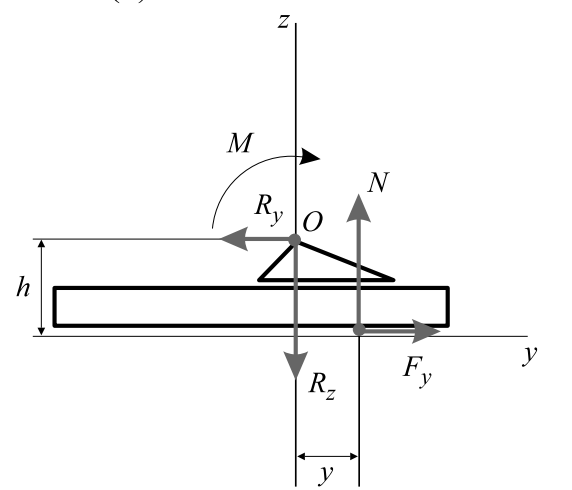
\includegraphics[width=0.5\linewidth]{foot.png}
    \caption{Силы действующие на на систему «стопы ног – платформа стабилоанализатора» }
    \label{fig:foot-platform}
\end{figure}

Где $F$ – это внешняя толкающая сила, $y$ – саггитальная координата центра давления, $l_1$ – высота точки к которой прикладывается толкающая сила
, $h$ – суммарная высота стопы и платформы стабилоанализатора, $N$ – нормальная реакция опоры

Ниже представлена система уравнений соответствующая рисунку \ref{fig:pendulum}
\begin{equation}\label{bodyforces}
    \left\{ {\begin{aligned}
                 & ml\ddot{\theta} = -R_y-F , \hfill                             \\
                 & 0=R_z-mg, \hfill                                              \\
                 & J \ddot{\theta} = mlg\sin \theta-Fl_1\cos \theta+M_x . \hfill \\
            \end{aligned}} \right.
\end{equation}
Проведем линеаризацию по $\theta$ в окрестности нуля
\begin{equation}\label{bodyforces}
    \left\{ {\begin{aligned}
                 & ml\ddot{\theta} = -R_y-F , \hfill             \\
                 & 0=R_z-mg, \hfill                              \\
                 & J \ddot{\theta} = mlg\theta-Fl_1+M_x . \hfill \\
            \end{aligned}} \right.
\end{equation}
Ниже представлена система уравнений соответствующая рисунку \ref{fig:foot-platform}
\begin{equation}\label{footforces}
    \left\{ {\begin{aligned}
                 & M_x = Ny+F_yh , \hfill \\
                 & F_y = R_y , \hfill     \\
                 & N \approx mg . \hfill  \\
            \end{aligned}} \right.
\end{equation}

Из \eqref{bodyforces} и \eqref{footforces} выразим $M_x$
$$M_x=mgy-h\left(F+ml\ddot{\theta}\right)$$

$$\left(J+mlh\right)\ddot{\theta}=mgl\theta+mgy-Fl_1-Fh$$


$$\frac{(J+mlh)l\ddot{\theta}}{mgl}=l\theta+y-\frac{F}{mg}(l_1+h);\quad $$
$$\text{Замена: }\eta=-l\theta; \quad T^2=\frac{J+mlh}{mgl};$$

\[
    T^2\ddot{\eta}=\eta-y+\frac{F}{mg}(l_1+h)
\]

\begin{equation}\label{eta_y}
    T^2\ddot{\eta}=\eta-(y-\frac{F}{mg}(l_1+h))
\end{equation}
Выражение \eqref{eta_y} можно свести к уравнению фильтра, путем корректировки входных данных $y$
\begin{equation}\label{eta_y_clear}
    T^2\ddot{\eta}=\eta-y
\end{equation}
Где $y$ - входные данные стабилоанализатора, $\eta$ выходные данные оценки координаты центра масс

В работе \cite{kruchPodoprihin} получено такое же уравнение для связи центра масс и центра давления. Показано, что его решение неустойчиво и приводит к катастрофическому нарастанию ошибки оценки на временах больше 0.5c.

Для использования предположения об отсутствии экспоненциальных составляющих, порожденных решением однородного уравнения, запишем передаточную функцию, соответствующую
уравнению \eqref{eta_y_clear}
\[
    G(s)=-\dfrac{1}{T^2s^2-1}
\]
В работе \cite{kruchPodoprihin} приведены два способа фильтрации данных: через преобразование Фурье и через фильрацию в прямом и обратном времени.

\section{Применение алгоритмов фильтрации к модельным данным}
модель со спиральной вовзвращающей силой, графики

Для оценки точности методов фильтрации проверим эти методы на модельных данных.
Пусть наша система задается уравнением
\[
    J\ddot{\theta}=m_Tgl\theta+M-Fl_1
\]
Где $M$ - момент в голеностопном суставе
Рассмотрим перевернутый маятник с спиральной пружиной в основании и вязким трением.
Получим следующее выражение
\begin{equation}\label{spiral_model}
    J\ddot{\theta}=mgl\theta-C\theta-P\dot\theta-Fl
\end{equation}
Где $C$ и $P$ неизвестные коэффиценты.
Подберем эти коэффиценты такими, чтобы \eqref{spiral_model} соответствовало затухающим колебаниям
с периодом $T\approx2c$
\begin{figure}[h!]
    \begin{center}
        \begin{minipage}[h]{0.48\linewidth}
            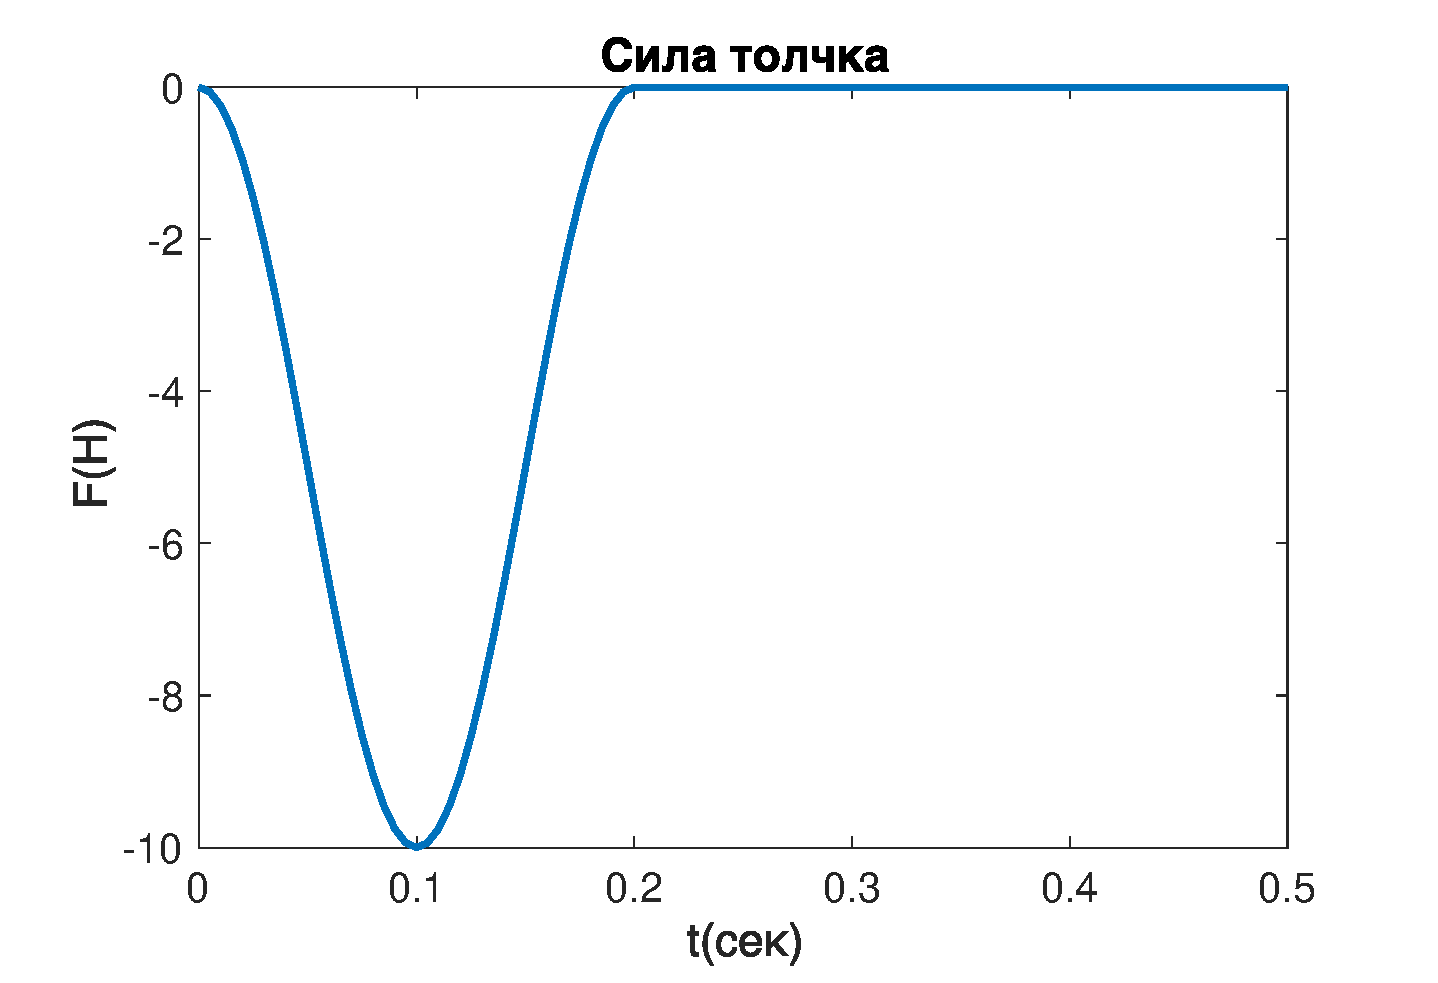
\includegraphics[width=1\linewidth]{push_model.eps}
            \caption{Пример зависимости \break $F(t)=5(1-\cos(4\pi\cdot2.5t))$}
        \end{minipage}
        \hfill
        \begin{minipage}[h]{0.48\linewidth}
            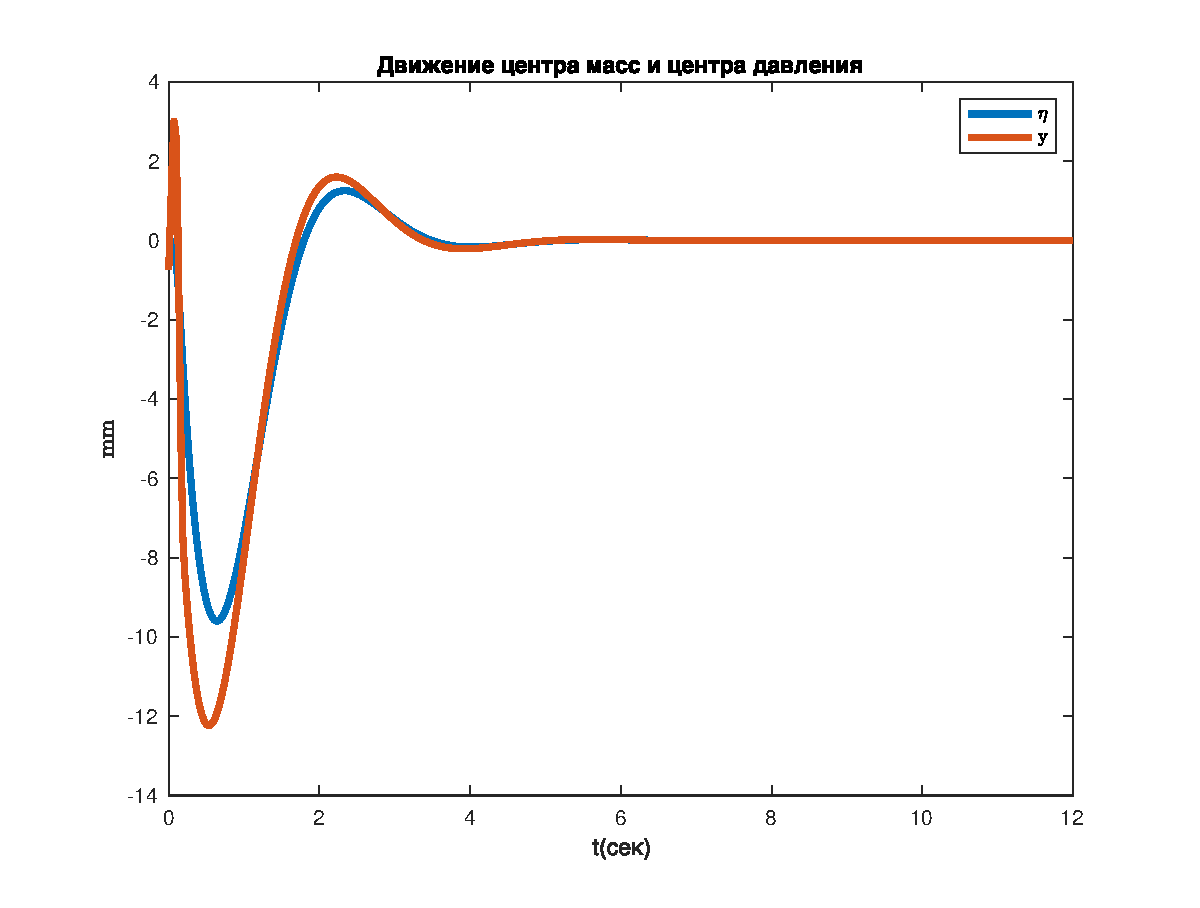
\includegraphics[width=1\linewidth]{eta_model.eps}
            \caption{Модельное движение центра масс и центра давления}
        \end{minipage}
    \end{center}
\end{figure}

Восстановим $\eta$ двумя способами
\begin{figure}[h!]
    \begin{center}
        \begin{minipage}[h]{0.48\linewidth}
            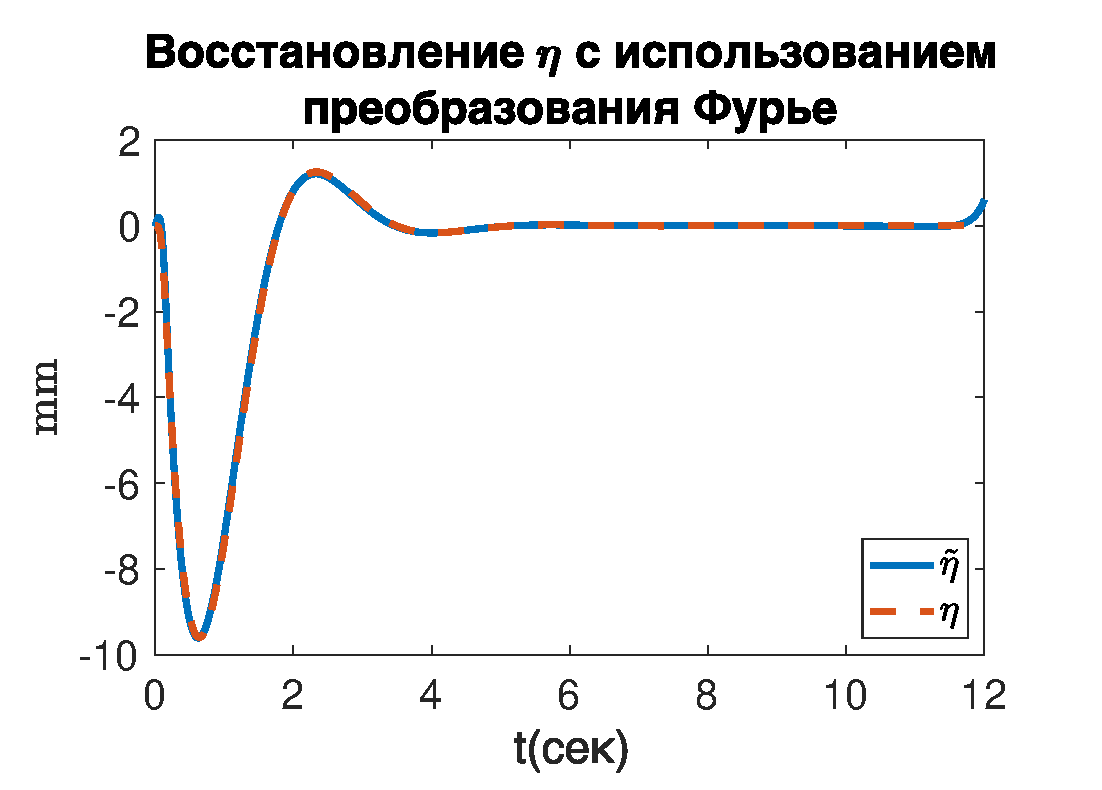
\includegraphics[width=1\linewidth]{eta_restore_fur_model.eps}
            \caption{Восстановление через преобразование Фурье}
        \end{minipage}
        \hfill
        \begin{minipage}[h]{0.48\linewidth}
            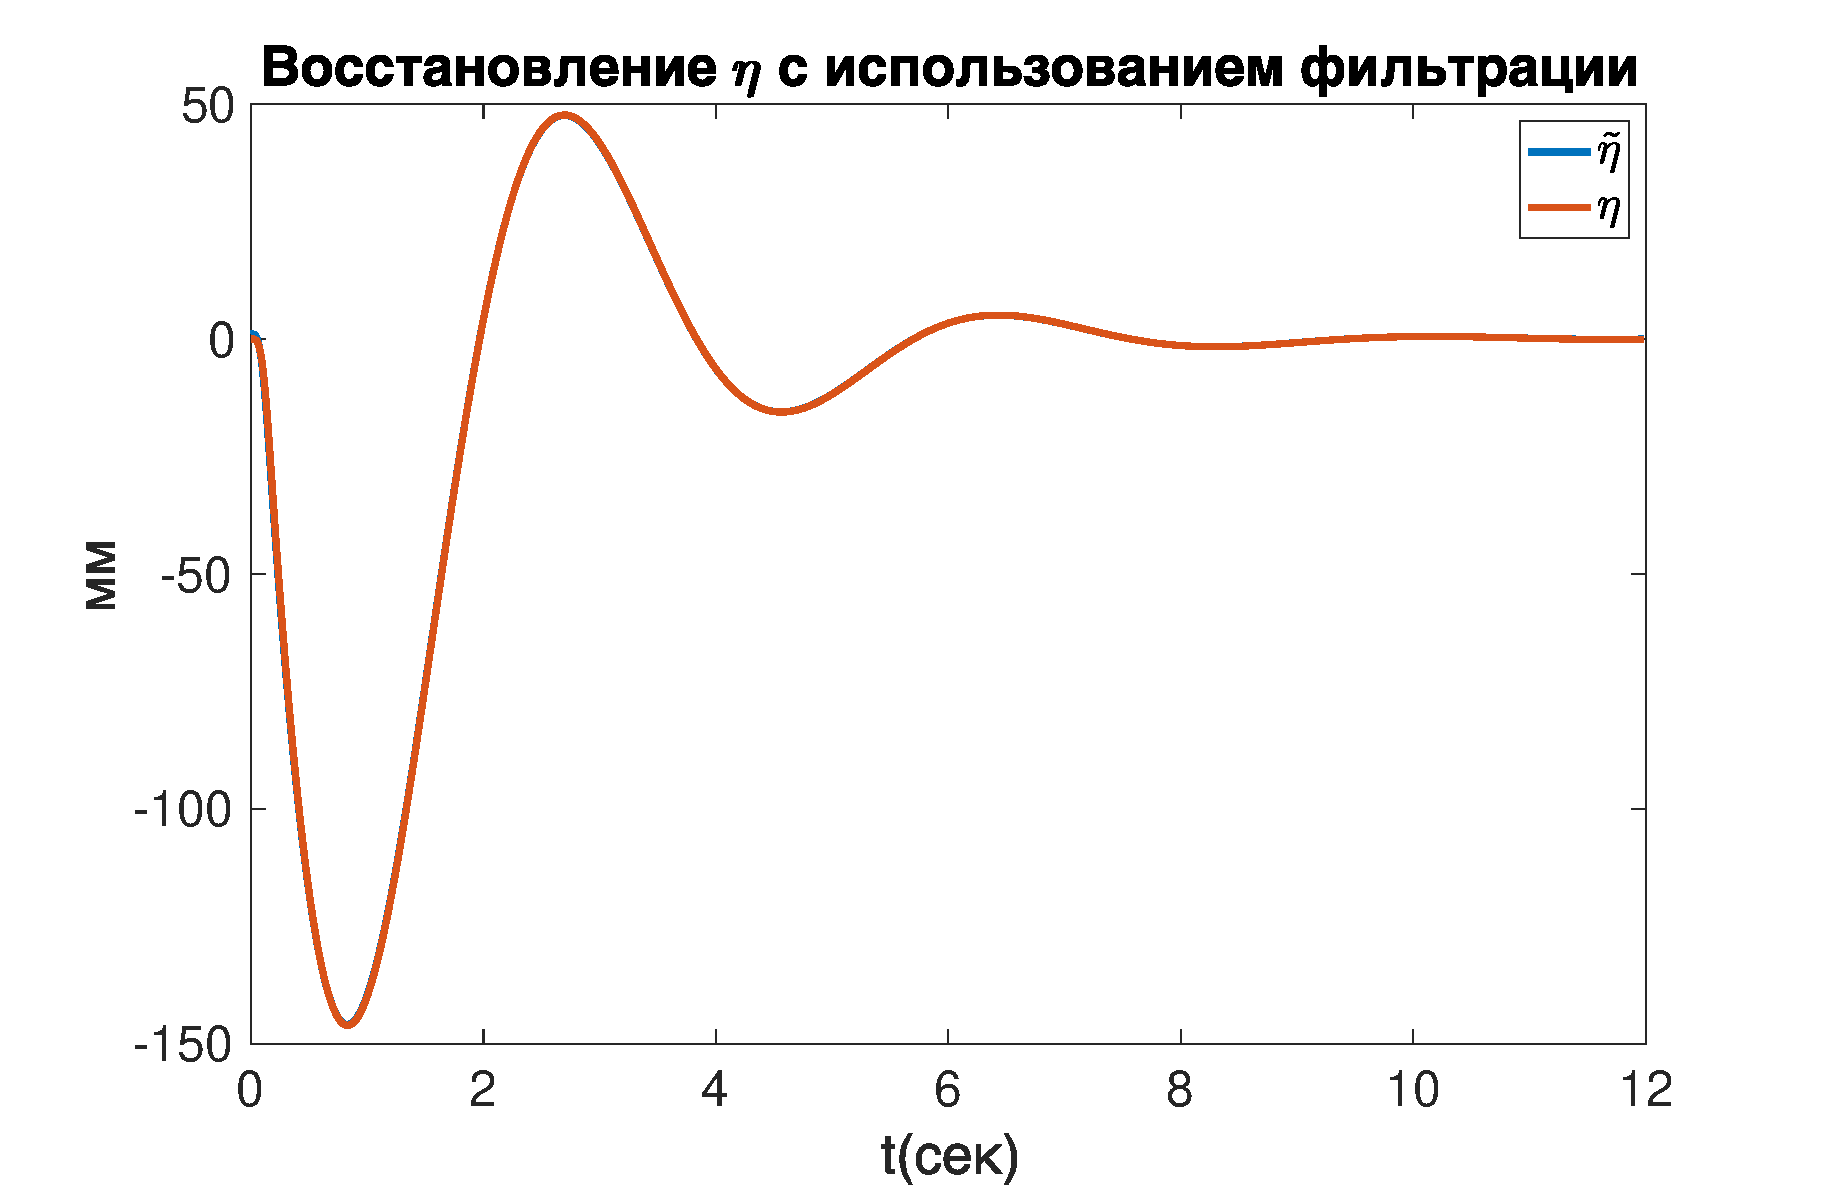
\includegraphics[width=1\linewidth]{double_filter_model.eps}
            \caption{Восстановление через двойную фильтрацию}
        \end{minipage}
    \end{center}
\end{figure}

Оценим полученные ошибки при восстановлении

\begin{figure}[h!]
    \begin{center}
        \begin{minipage}[h]{0.48\linewidth}
            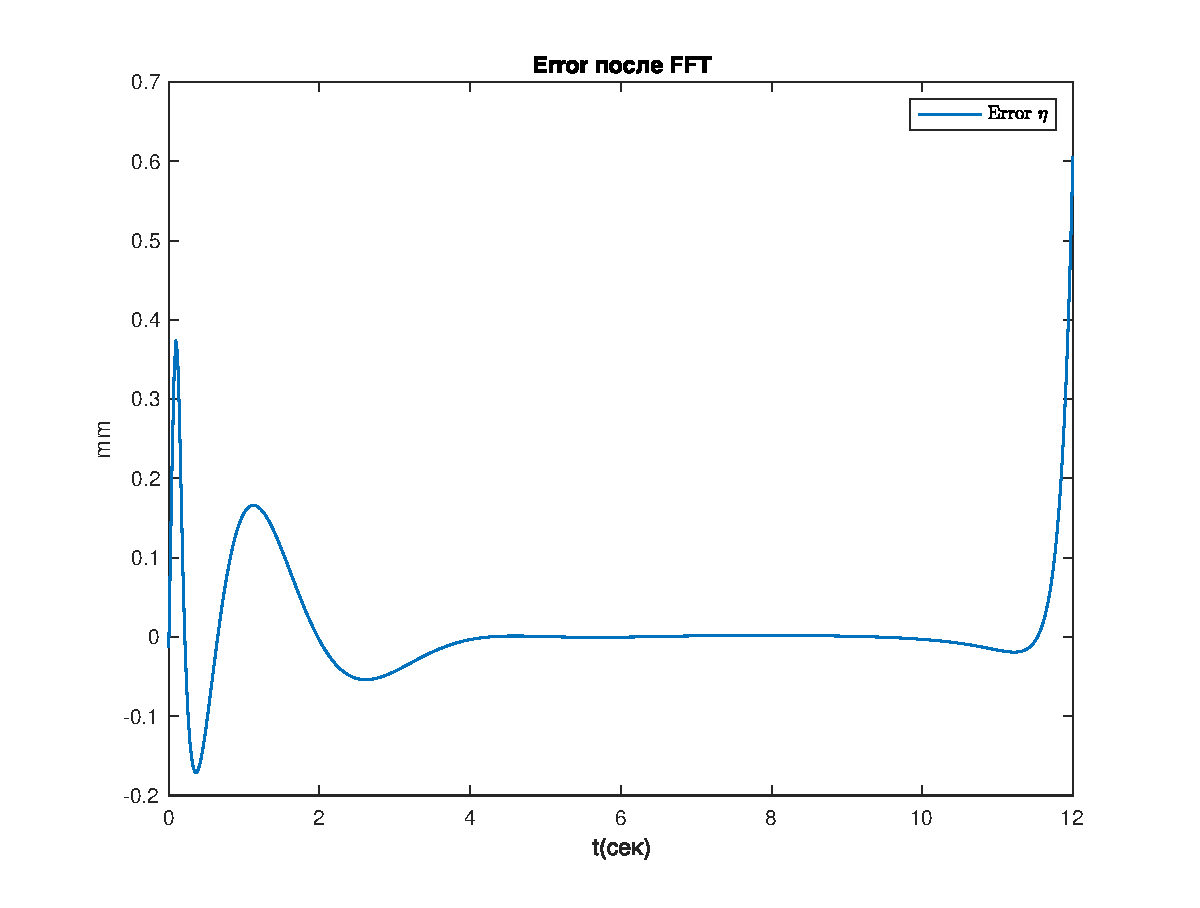
\includegraphics[width=1\linewidth]{err_furier_model.eps}
            \caption{Ошибка восстановления через преобразвоание Фурье ,rmse=0.0761}
        \end{minipage}
        \hfill
        \begin{minipage}[h]{0.48\linewidth}
            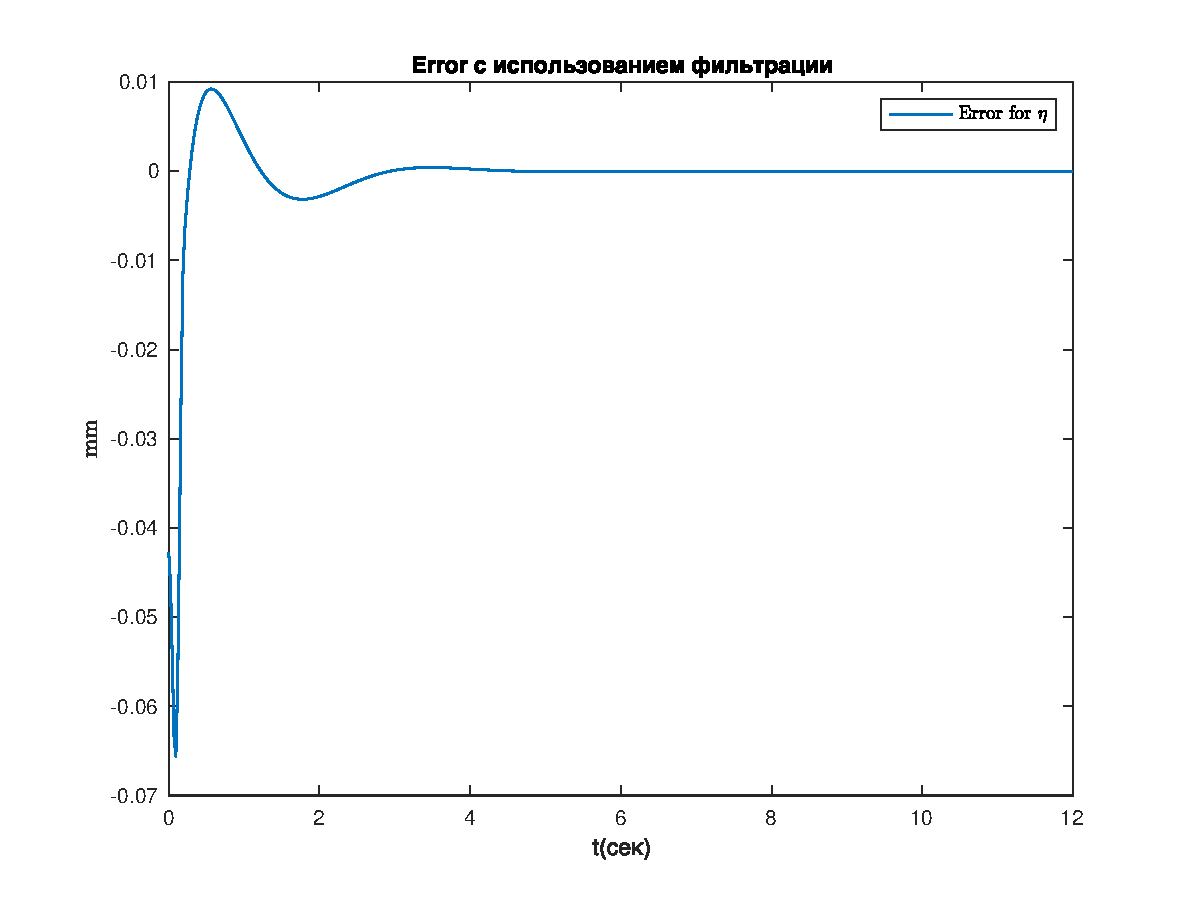
\includegraphics[width=1\linewidth]{err_double_filter_model.eps}
            \caption{Восстановление через двойную фильтрацию, rmse=0.0061}
        \end{minipage}
    \end{center}
\end{figure}

\todo[inline]{ошибка/макс модуль отклонения}

Погрешности обоих методов очень небольшие, почти идеально восстанавливают исходную траекторию центра масс

\section{Анализ данных со стабилоанализатора и силомера}
\todo[inline]{оценка времени где толчки были, сила берем крутой/пологий спуск}

Оценим массу, на рисунках \ref{mass_full_time} и
\ref{mass_short_time} представлены графики показаний массы испытуемого человека

\begin{figure}[h!]
    \begin{center}
        \begin{minipage}[h]{0.46\linewidth}
            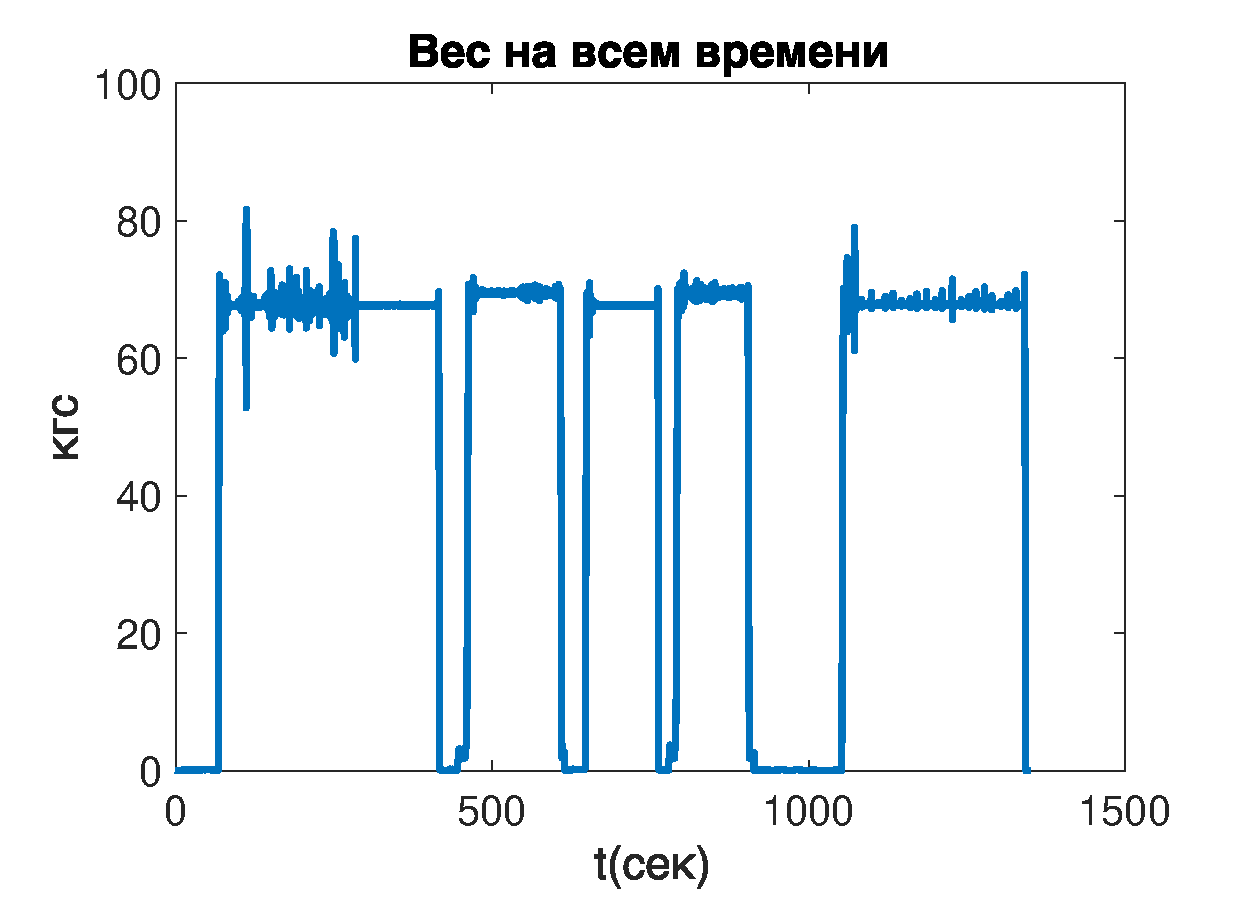
\includegraphics[width=1\linewidth]{mass_full_time.eps}
            \caption{Масса на всем интервале наблюдений}
            \label{mass_full_time}
        \end{minipage}
        \hfill
        \begin{minipage}[h]{0.46\linewidth}
            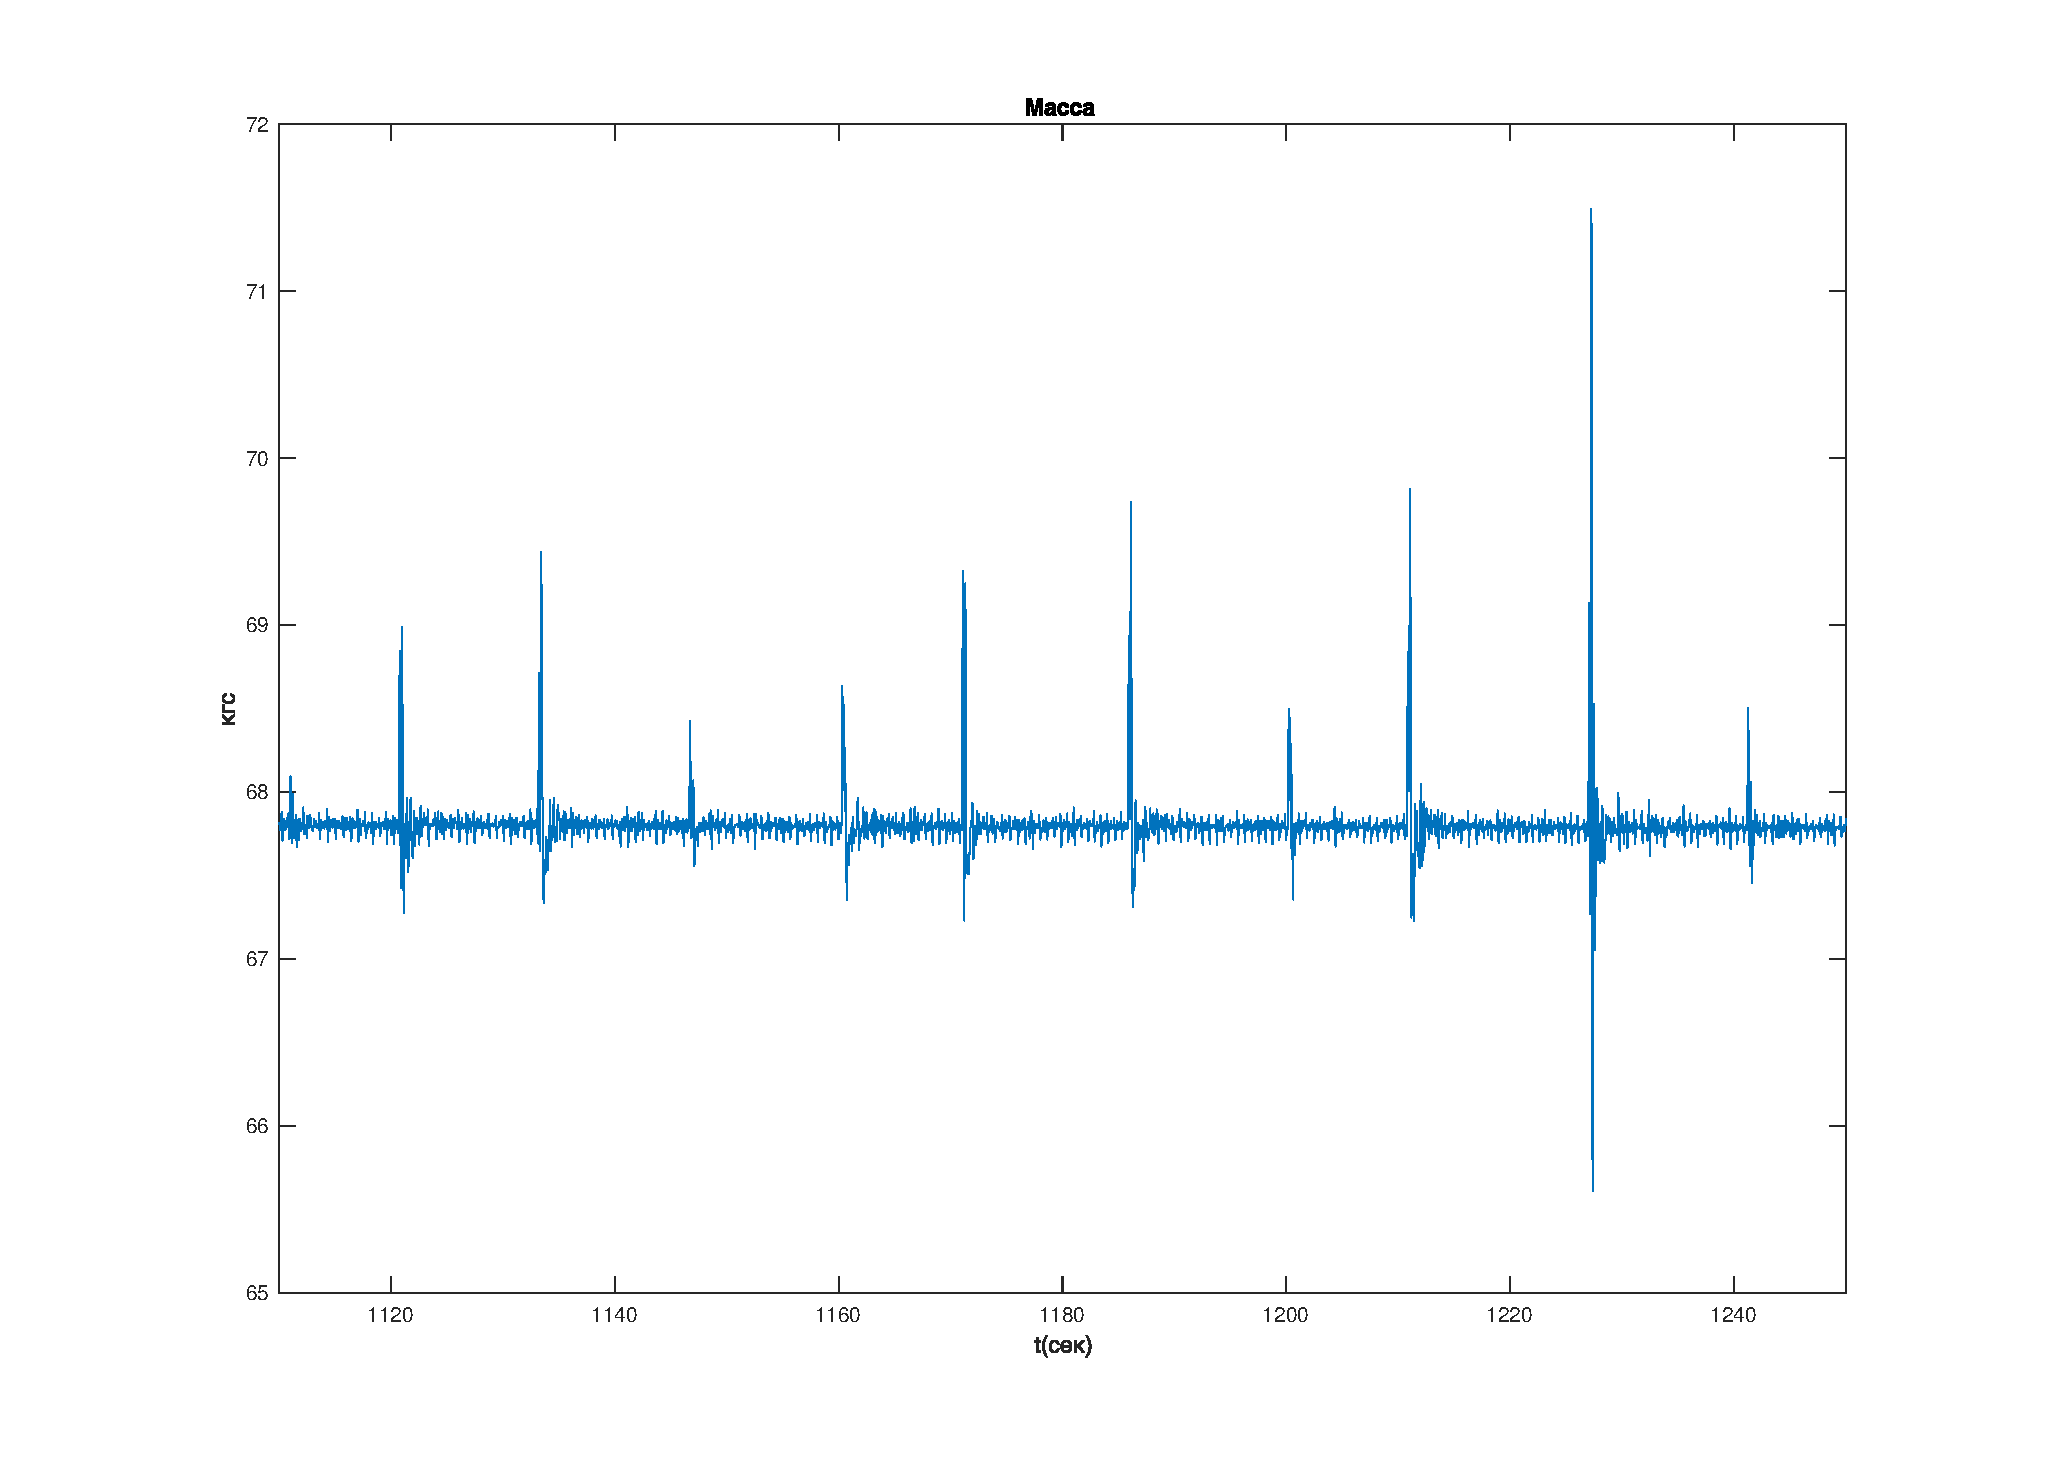
\includegraphics[width=1\linewidth]{mass_concrete.eps}
            \caption{Масса на интервале исследуемых толчков}
            \label{mass_short_time}
        \end{minipage}
    \end{center}
\end{figure}

Среднее значение рассчитаем по рисунку \ref{mass_short_time}, $m=67.8$кг

Проанализируем силу толчков (см. рис. \ref{pushes_real}), сила толчка колеблется от 1 до 10 Н,
в первую очередь возьмем толчки большей силы, так как на них предположительно лучше удастся провести исследование.

\begin{figure}[h!]
    \centering
    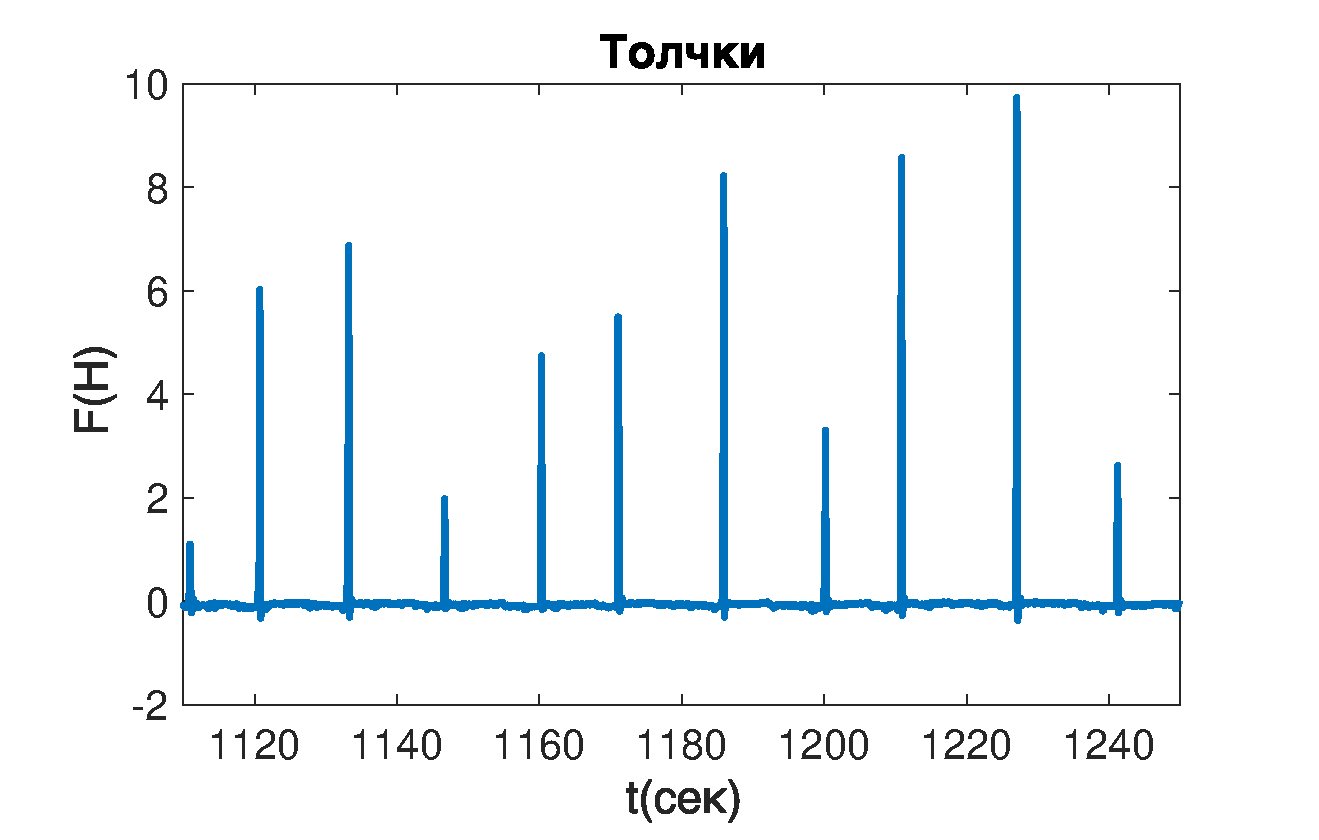
\includegraphics[width=0.9\linewidth]{pushes_real.eps}
    \caption{Силовое воздействие на интервале наблюдения}
    \label{pushes_real}
\end{figure}

\begin{figure}[h!]
    \centering
    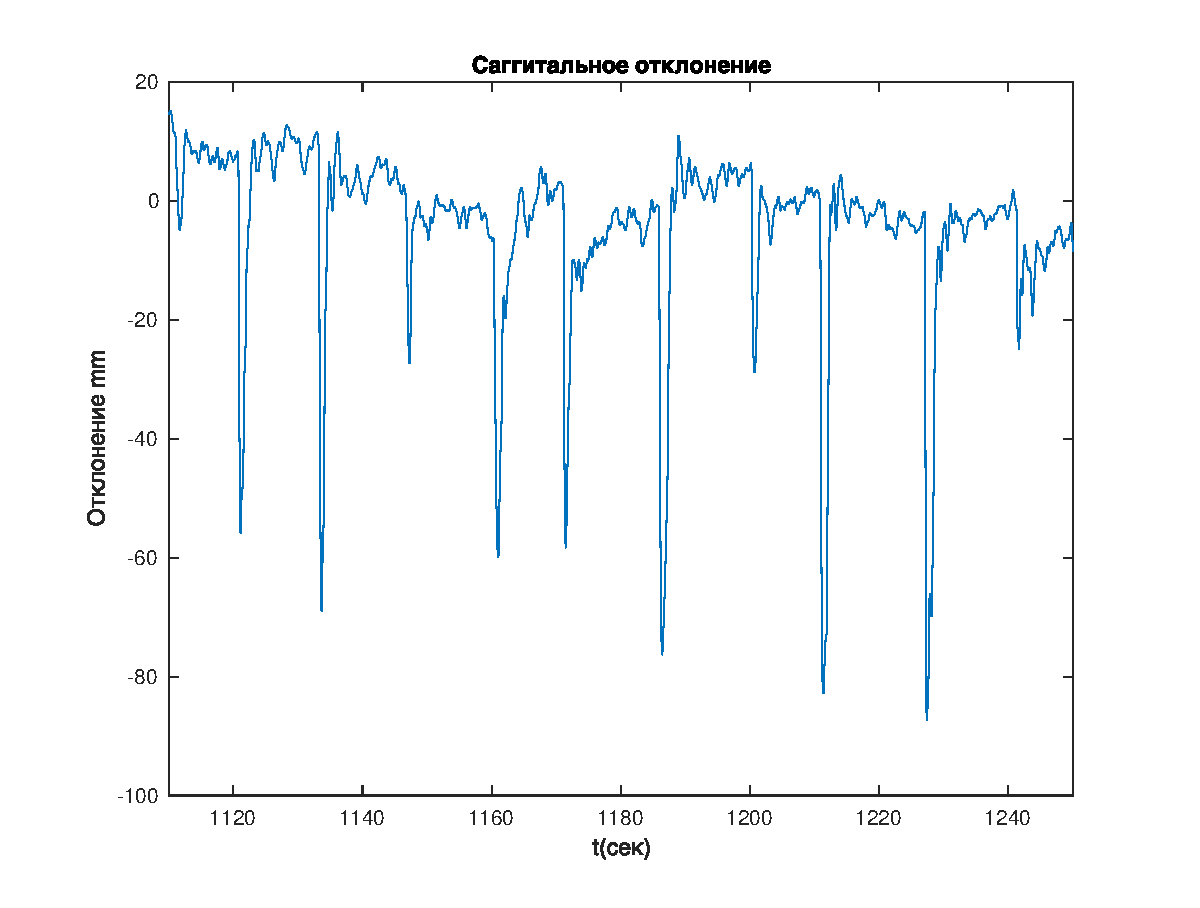
\includegraphics[width=0.9\linewidth]{y_real.eps}
    \caption{Саггитальное отклонение центра давления при толчках}
    \label{y_real}
\end{figure}



\section{Применение алгоритмов фильтрации к экспериментальным данным}
Рассмотрим один конкретный толчок (около момента времени 1120) и для него применим два способа
фильтрации (см. рис. \ref{restore_double_real} и \ref{restore_fur_real})

\begin{figure}[h!]
    \centering
    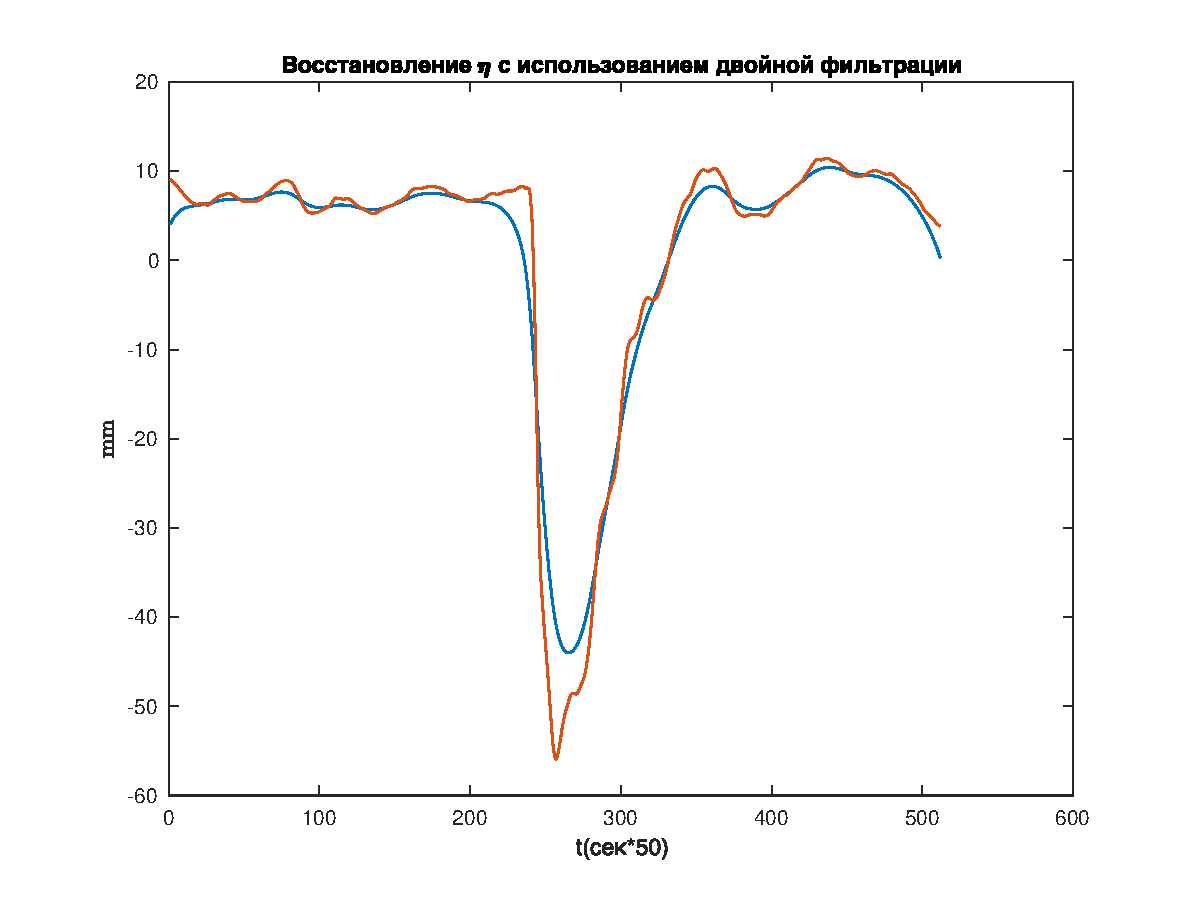
\includegraphics[width=0.65\linewidth]{restore_eta_double_real.eps}
    \caption{Восстановление с использованием двойной фильтрации}
    \label{restore_double_real}
\end{figure}

\begin{figure}[h!]
    \centering
    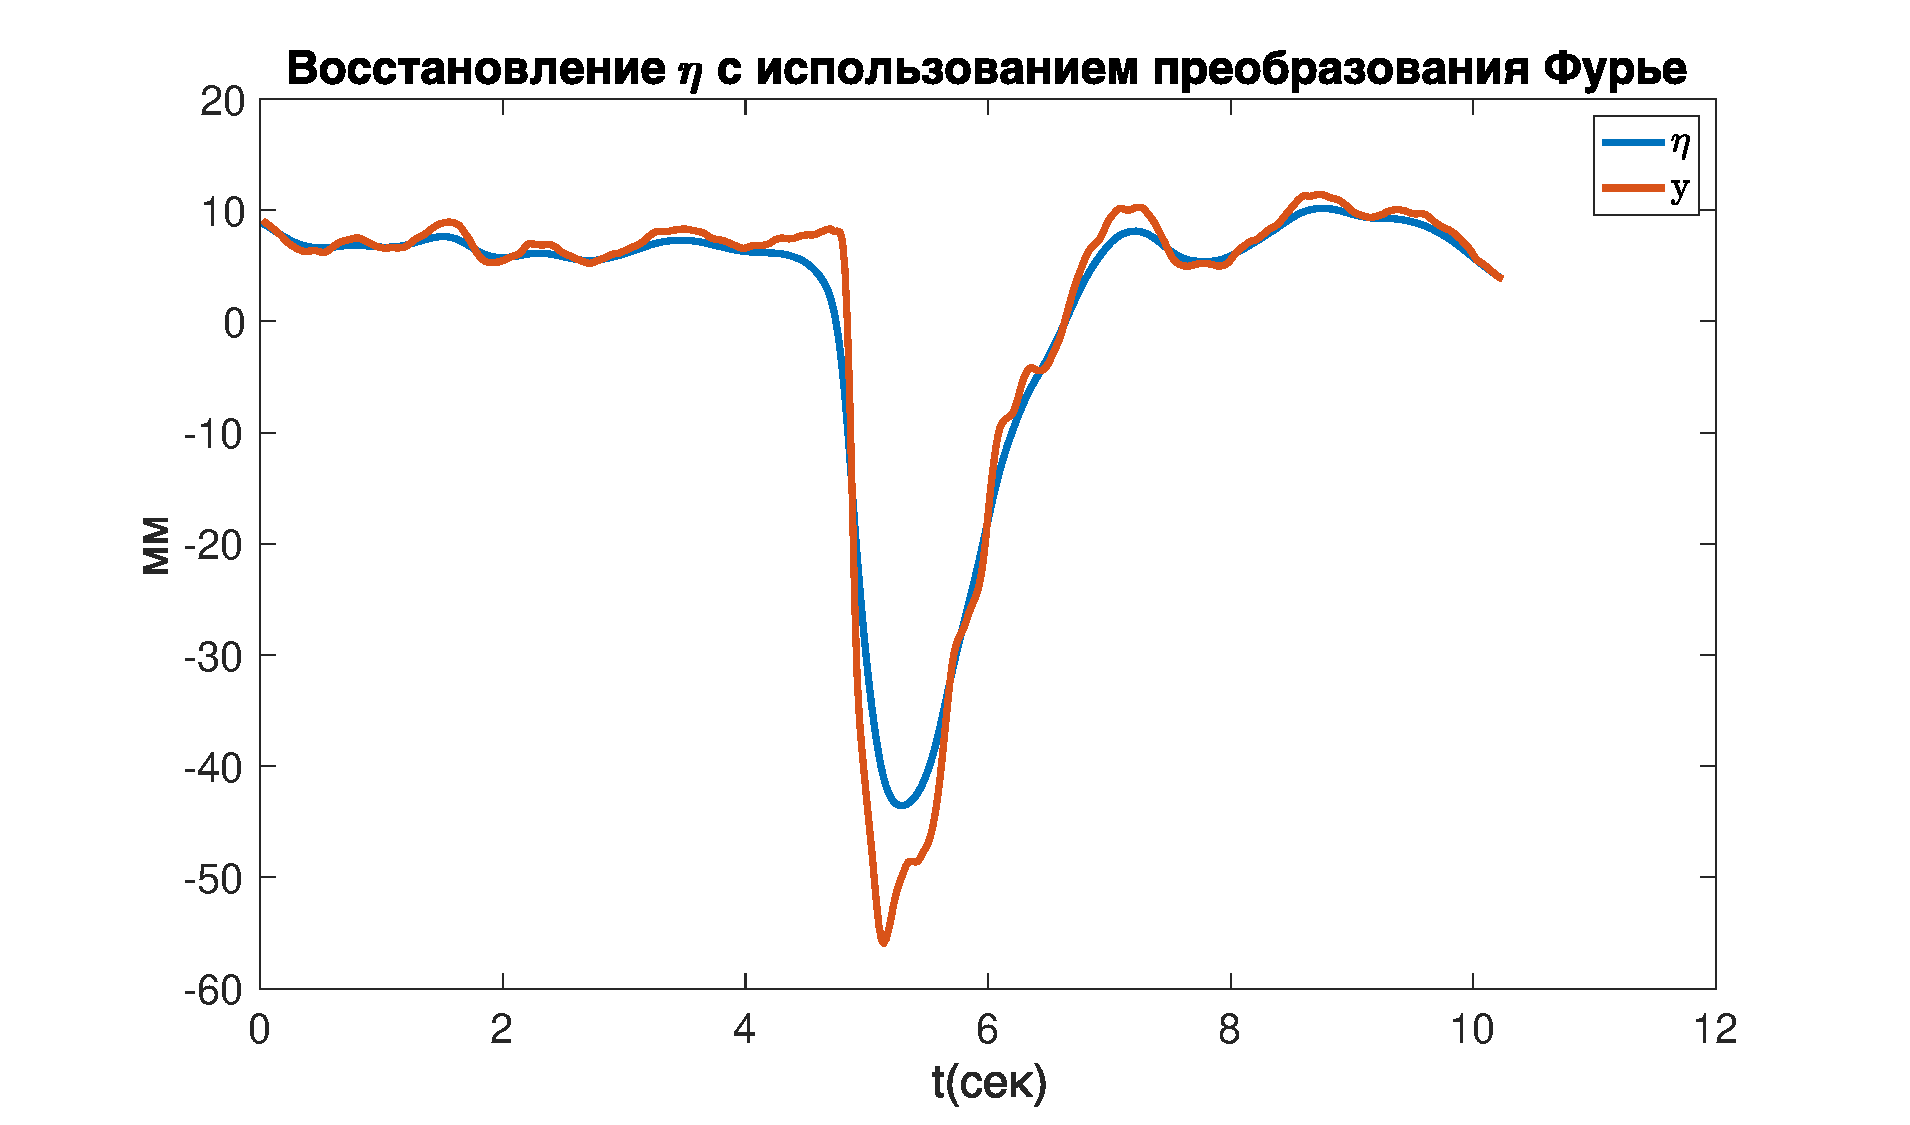
\includegraphics[width=0.65\linewidth]{restore_eta_fur_real.eps}
    \caption{Восстановление с использованием преобразования Фурье}
    \label{restore_fur_real}
\end{figure}

Визуально видно, что ожидаемая и полученная траектория центра масс совпадают,
без каких-либо аномальных отклонений

\section{Оценка начальных условий в моменты завершения толчков}

В задаче быстродейтсвия присутсвует несколько неизвестных параметров:

$m_T$ -  масса тела человека, $u_*$ - модуль оптимального управления,
$t_*$ - коэффицент обезразмеривания времени,
$\varphi_*\approx\varphi_0$ - характерное значение угла отклонения тела

$m_T=67.8$кг

$l=0.88$м

$$t_\ast=\sqrt{\frac{J}{m_Tgl}}=\sqrt{\frac{1/3 \cdot m_T l^2}{m_Tgl}}=\sqrt{\frac{l}{3g}}$$
\[
    u^-=\frac{t_\ast U^-}{mgl\varphi_\ast },\ \ u^+=\frac{t_\ast U^+}{mgl\varphi_\ast}.
\]
$|U^+|=|U^-|=\dot M\approx \Delta M \cdot \nu, \text{ где } \nu - \text{частота дискретизации данных на стабилоанализаторе } $
$\nu =50\text{Гц}$

В работе \cite{kruchinMetoda} показано, что $\Delta y=\dfrac{\Delta M}{mg}$.

Возьмем 5 толчков и по ним определим средний возникающий момент в голеностопе см. таблицу \ref*{moments_calculating}
% Please add the following required packages to your document preamble:

\begin{table}[h!]
    \centering
    \begin{tabular}{@{}|l|c|c|c|l|@{}}
        \toprule
          & \multicolumn{1}{l|}{xStart(сек)} & \multicolumn{1}{l|}{xEnd(сек)} & \multicolumn{1}{l|}{$\Delta Y$(мм)} & \multicolumn{1}{l|}{$\Delta M $(Н $\cdot$ м)} \\ \midrule
        1 & 1098.9                           & 1099.3                         & 64.7                                & 43.1                                          \\ \midrule
        2 & 1120.8                           & 1121.0                         & 61.5                                & 40.9                                          \\ \midrule
        3 & 1133.2                           & 1133.6                         & 72.6                                & 48.3                                          \\ \midrule
        4 & 1185.9                           & 1186.2                         & 65.18                               & 43.4                                          \\ \midrule
        5 & 1277.8                           & 1278.0                         & 67.3                                & 44.7                                          \\ \bottomrule
    \end{tabular}
    \caption{Данные для расчета возникающего момента в голеностопе, см. рис. \ref{y_real} }
    \label{moments_calculating}
\end{table}

Среднее значение $\Delta M=44.07$ Н$\cdot$м

Среднее значение $U^+=\dfrac{\Delta M}{\Delta t}=144.7$ Н$\cdot$м/c $,\Delta t_i=xEnd_i-xStart_i$
\begin{figure}[h!]
    \centering
    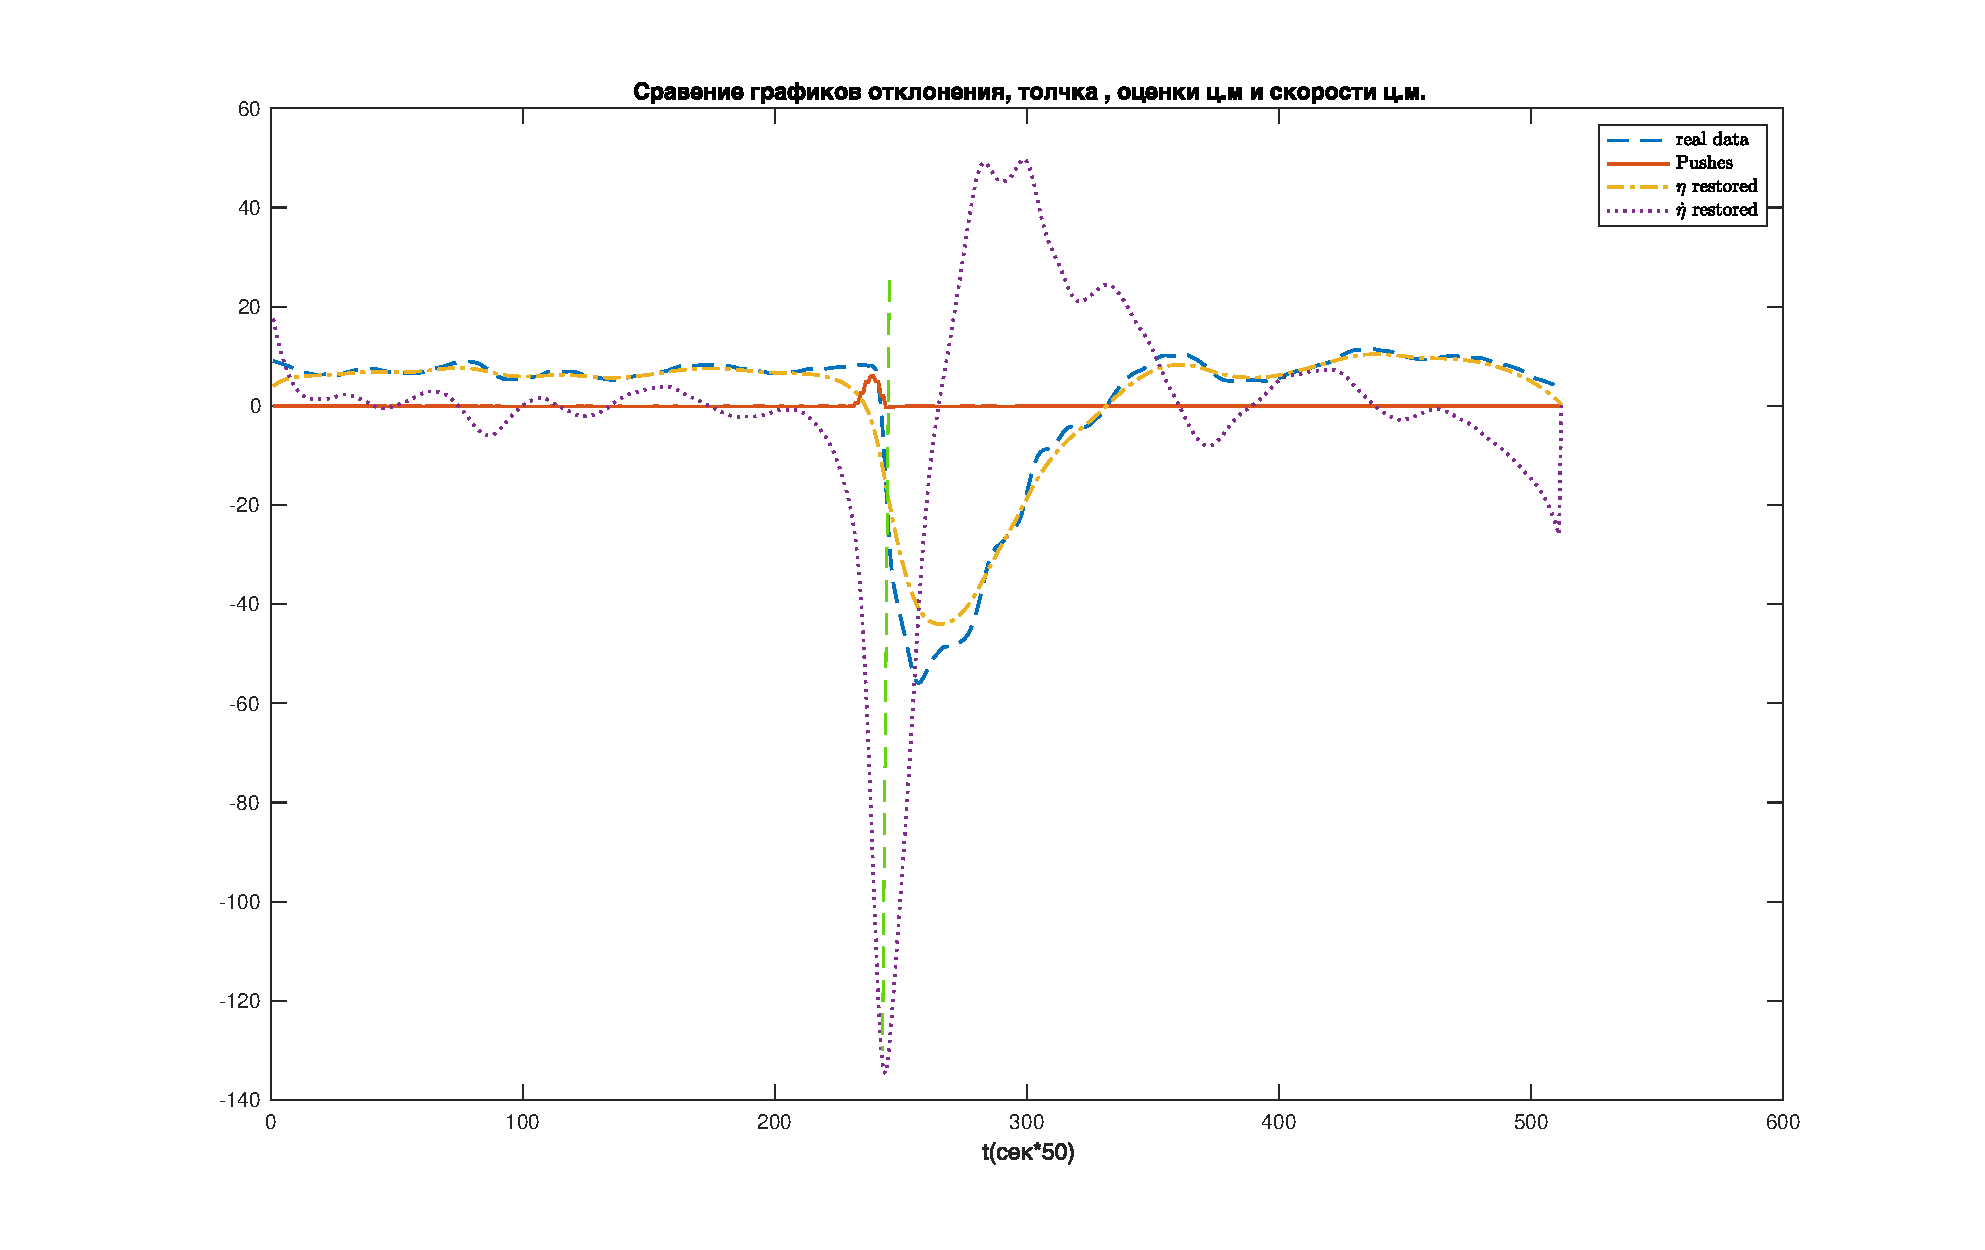
\includegraphics[width=0.65\linewidth]{all_real.eps}
    \caption{Определение начальных условий в момент завершения толчка}
    \label{all_real}
\end{figure}

На рисунке \ref{all_real} представлены графики исходных данных, данные силомера, восстановленая траектория центра масс и ее первая производная, вычисленная как первая разность, умноженная на частоту дискретизации.

Вертикальная ось - Н, мм, мм/с для соответствующих величин. Момент завершения толчка соответствует точке с абсциссой 245. В ней берем начальные условия:

$\varphi_0=0.0292,\quad \omega_0=0.1490$

На основе которых можем уже решать задачу быстродействия

\newpage

\chapter{Анализ полученных решений задачи быстродействия}

\section{Сравнение траекторий и времени возвращения для выборки толчков}

\todo[inline]{корректировка траектории (offset/linear trend)
    картинки с траекториями, много, берем u=3.2 3.6 наиболее подходящее
    таблички, отношения времен real/opt}
Посчитаем безразмерное $u_\ast$

\[
    u_\ast=\frac{t_\ast U^-}{mgl\varphi_\ast }=1.46
\]
При таком значении действительных корней уравнения \eqref{final_polynom} больших 1 нет,
при обоих комбинациях знаков $u_\ast$.

Объяснение этому явлению такое: нервная система успела за время толчка среагировать и в голеностопе уже возник возвращающий момент, который не даст человеку упасть.
Но в нашей постановке задачи, считается, что момент не успел возникнуть. Для корректировки завысим значение $u_\ast$ в $2-3$ раза.

\begin{figure}[h!]
    \centering
    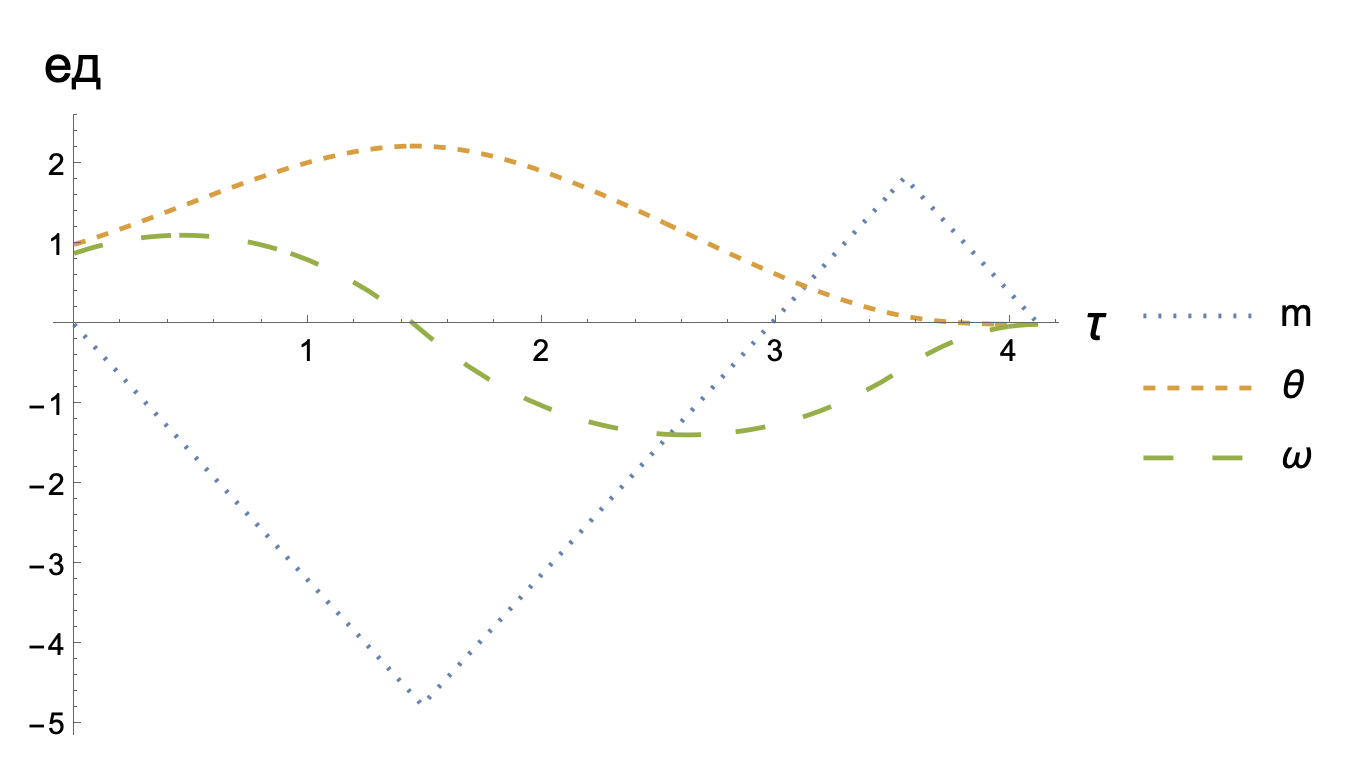
\includegraphics[width=0.7\linewidth]{3_graphs.png}
    \caption{Оптимальная траектории в безразмерном виде $u=3.2$ }
    \label{3_graphs}
\end{figure}

Посторим полученные траектории для различных значений $u_\ast$(см. рис. \ref{final_graphs}, \ref{final_graphs_1}).

Данные со стабилоанализатора, содержат погрешности, спокойное
положение немного блуждает, поэтому скорреткируем координаты
центра масс, на ее среднее значение до и после толчка. Корректировка представляет собой аналог
 вычитания линейного тренда.
\begin{figure}[h!]
    \centering
    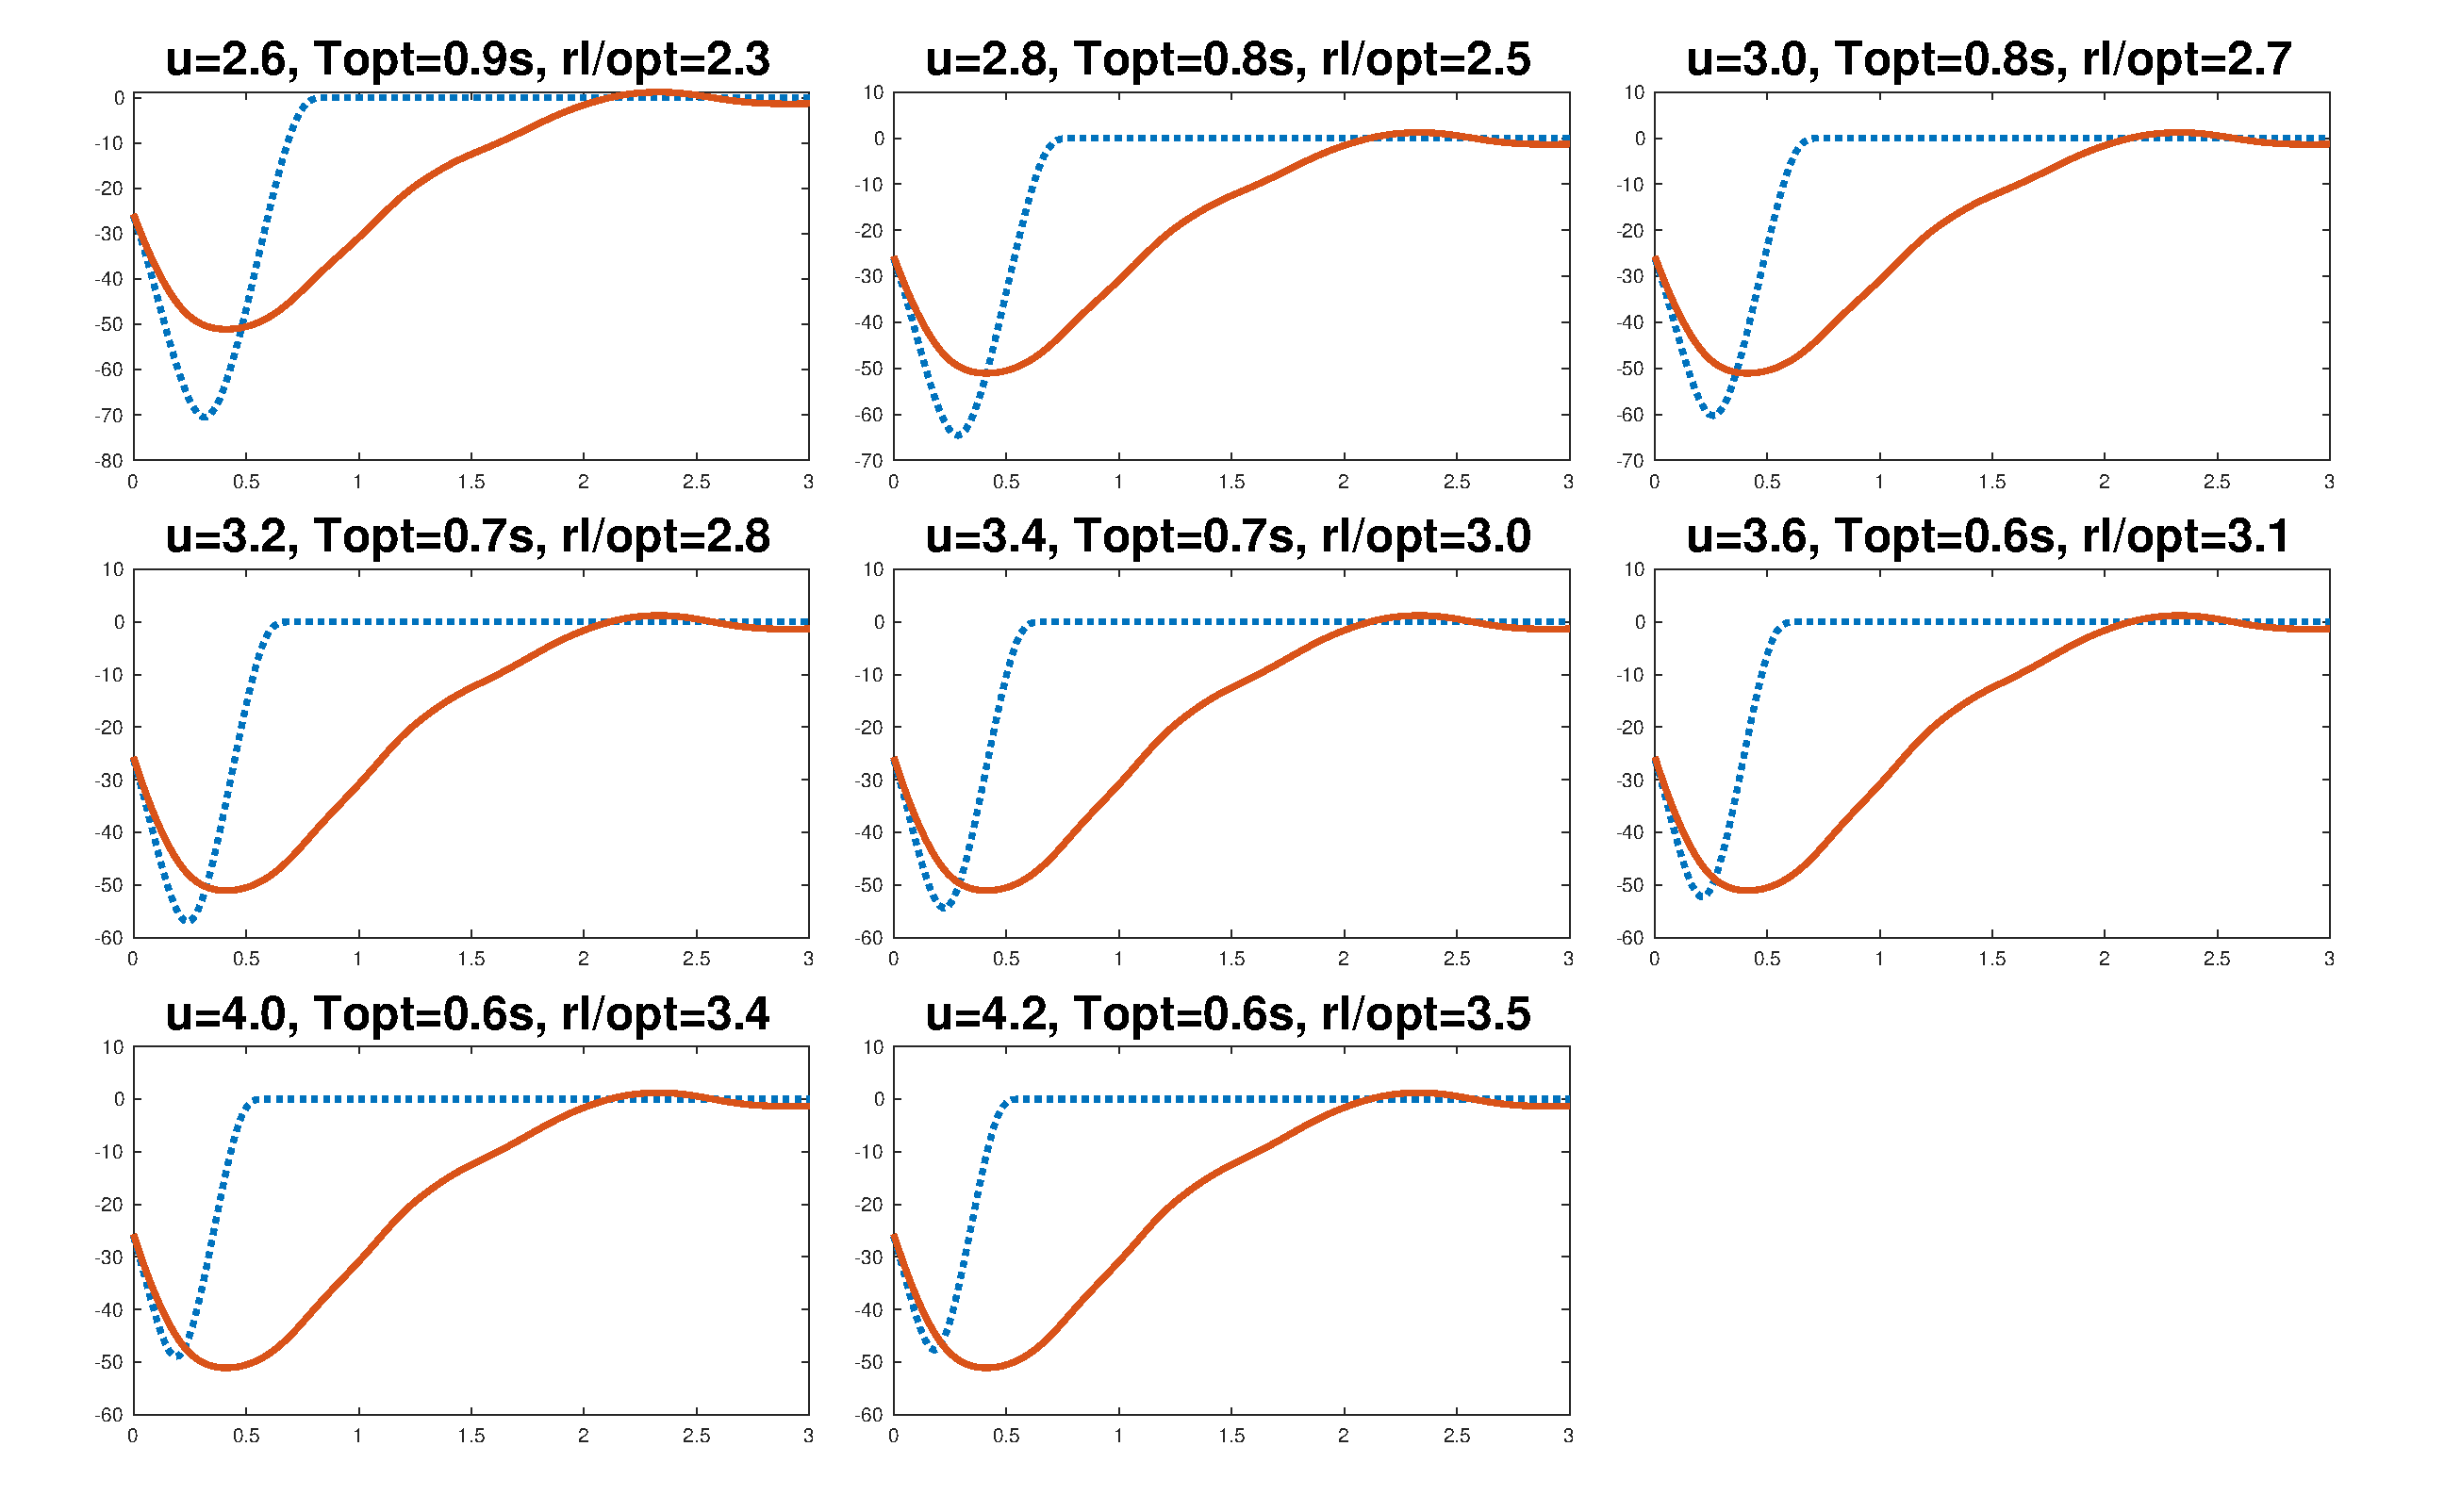
\includegraphics[width=1\linewidth]{final_graphs.eps}
    \caption{Оптимальные(голубые) и реальные(оранжевые) траектории на возвратном движении человека отметка 1120}
    \label{final_graphs}
\end{figure}

\begin{figure}[h!]
    \centering
    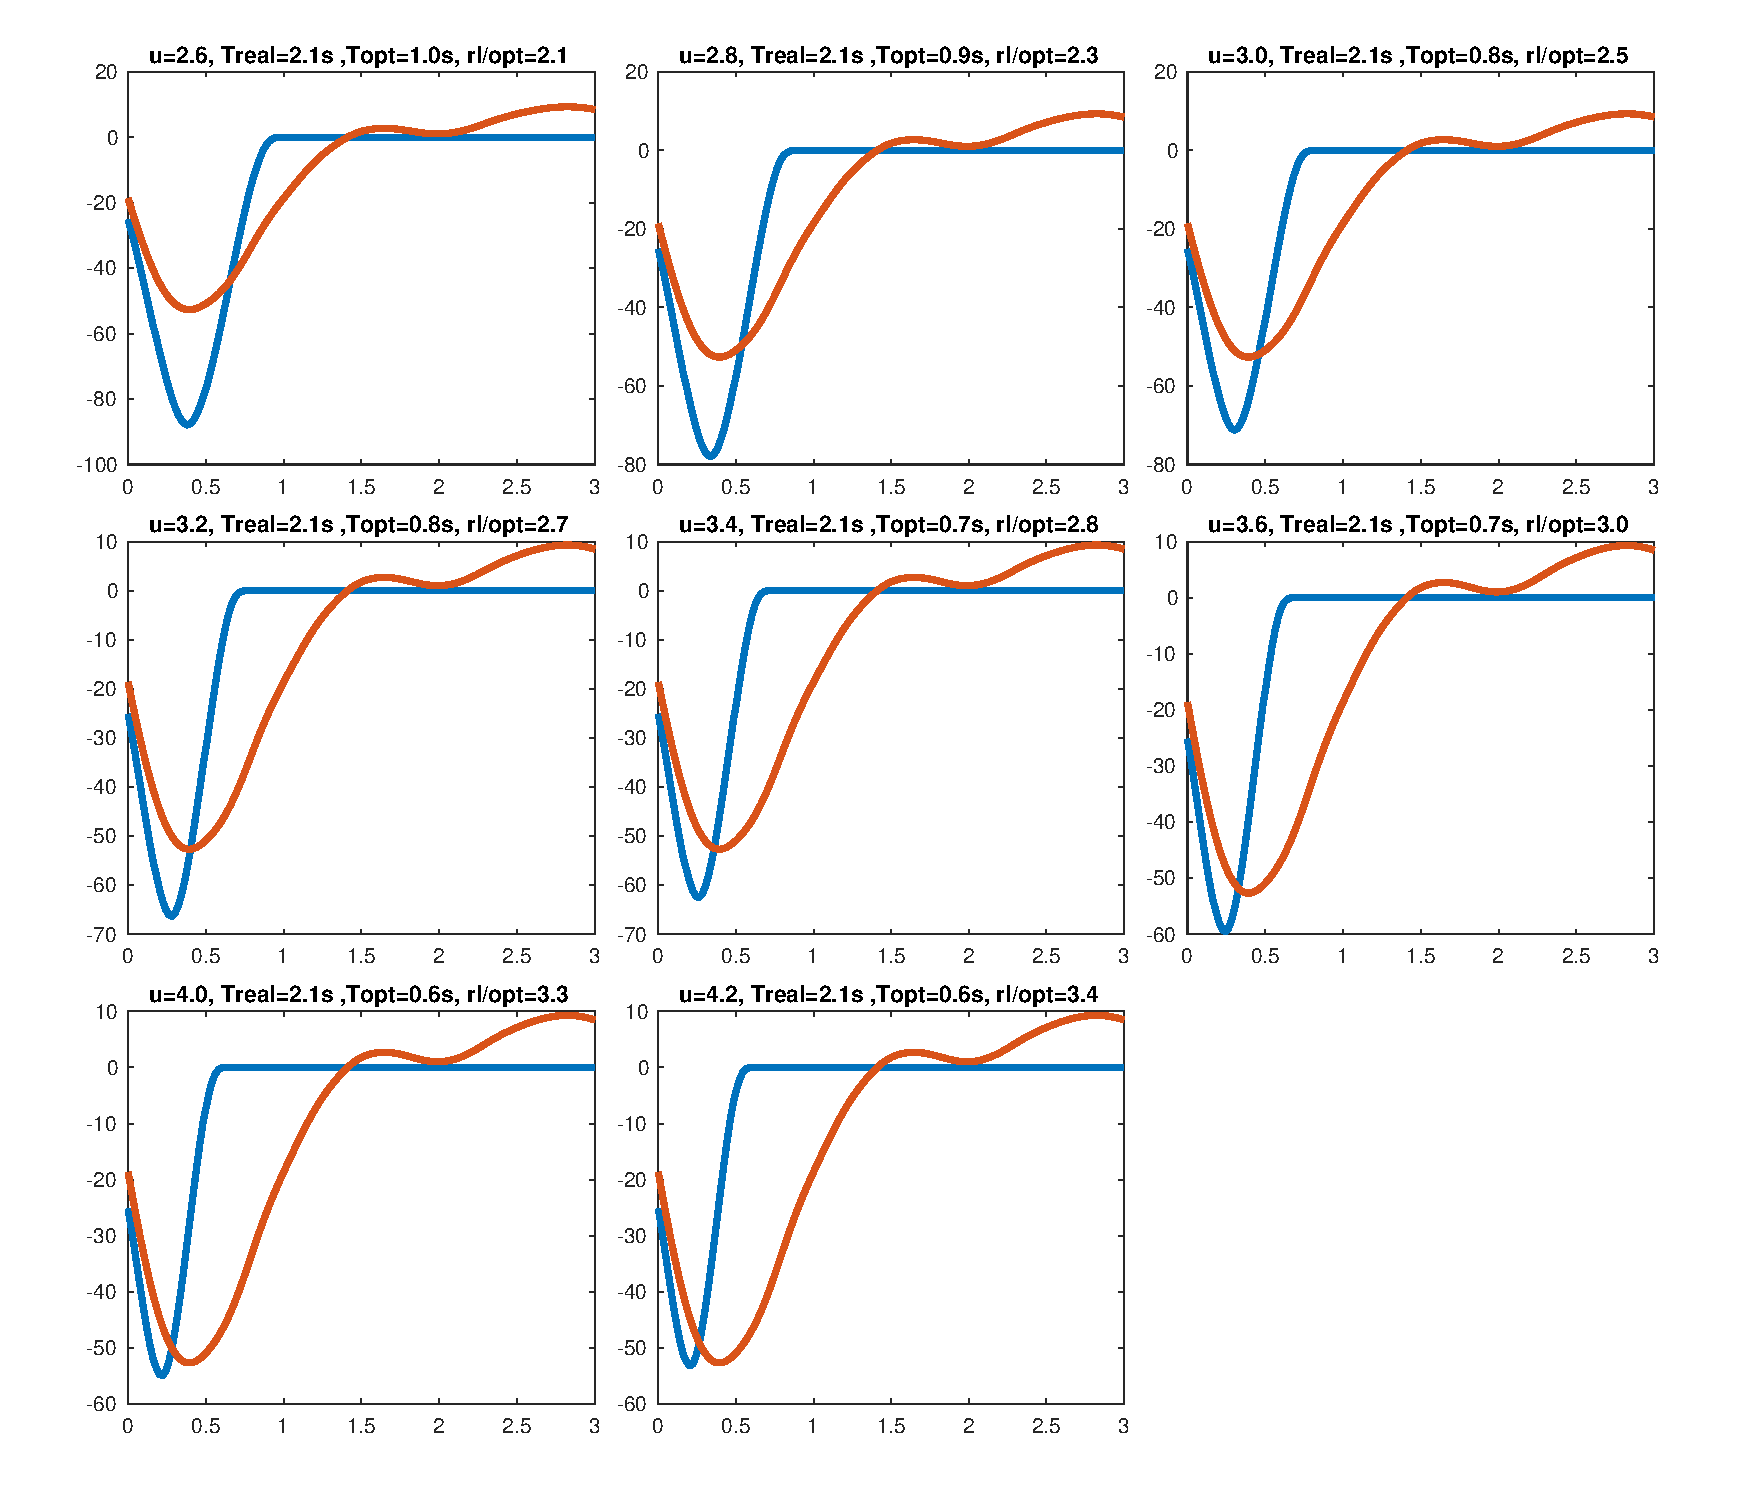
\includegraphics[width=1\linewidth]{final_graphs_1.eps}
    \caption{Оптимальные(голубые) и реальные(оранжевые) траектории на возвратном движении человека отметка 1130}
    \label{final_graphs_1}
\end{figure}

Проведем аналогичный анализ для нескольких толчков,
 результаты представлены в таблице \ref{final_table}.

\todo[inline]{анализ таблицы}
 
 \begin{table}[h!]
    \centering
    \begin{tabular}{|l|c|c|c|c|c|c|c|c|c|}
    \hline
    \textbf{Номер толчка} & \textbf{1} & \textbf{2} & \textbf{3} & \textbf{4} & \textbf{5} & \textbf{6} & \textbf{7} & \textbf{8} & \textbf{9} \\ \hline
    \textbf{$F_{max}$(Н)}       & 6.01  & 6.87  & 8.21  & 8.56  & 9.73  & 4.74  & 5.49  & 1.97  & 3.3   \\ \hline
    \textbf{Время толчка(сек)}  & 0.26  & 0.26  & 0.26  & 0.26  & 0.26  & 0.26  & 0.26  & 0.26  & 0.26  \\ \hline
    \textbf{$\varphi_0$}           & 0.026 & 0.028 & 0.033 & 0.033 & 0.035 & 0.022 & 0.018 & 0.008 & 0.007 \\ \hline
    \textbf{$\omega_0$}   & 0.1490     & 0.1767     & 0.1689     & 0.1955     & 0.2139     & 0.0989     & 0.1453     & 0.0513     & 0.0786     \\ \hline
    \textbf{Момент(кг*м)}       & 14.88 & 19.21 & 17.95 & 19.28 & 19.95 & 9.97  & 14.16 & 6.38  & 7.95  \\ \hline
    \textbf{real/opt $u_*=3.2$} & 2.8   & 2.7   & 2.8   & 2.8   & 2.9   & 2.7   & 1.8   & 1.8   & 2.0   \\ \hline
    \textbf{real/opt $u_*=3.6$} & 3.1   & 3.0   & 3.1   & 3.1   & 3.2   & 2.9   & 2.0   & 2.0   & 2.3   \\ \hline
    \end{tabular}
    \caption{Анализ различных толчков}
    \label{final_table}
    \end{table}

\section{Гипотезы по корректировке задачи}
момент успел измениться, не максимальное а какое-то другое управление


\newpage


\chapter*{Заключение}

\addcontentsline{toc}{chapter}{Заключение}

\todo[inline]{Похоже немного на оптимальную траекторию, но много допущений, момент уже успел измениться, видимо мышцы не совсем так работают, нужны уточнения задачи, с различными постановками.
    Управление взять в каком-то интервале, а так в целом хорошо построил решение.}

В дипломной работе были представлены оптимальные алгоритмы управления
движением позой при ступенчатом воздействии, основанные на модели
«перевернутого маятника» удовлетворяющие принципу максимума Понтрягина.
В задаче ставилось ограничение на скорость изменения момента в голеностопном суставе.
\begin{itemize}
    \item Показано, что решение оптимальной задачи быстродействия при ограниченной скорости изменения момента в голеностопном суставе может иметь решение, которое хорошо качественно совпадает с картиной, наблюдаемой в стабилометрических исследованиях.
    \item Время необходимое для восстановления исходной позы получилось соизмеримым с реальным времени возвращения после толчка.
\end{itemize}




\newpage

\addcontentsline{toc}{chapter}{Литература}

\begin{thebibliography}{15}
    \bibitem{pandy}Pandy M.G., Zajac F.E., Sim E., Levine W.S. An optimal control model for maximum height human jumping// Journal of Biomechanics.-1990, vol. 23 – pp.1185-1198.
    \bibitem{humanMovements}Happee R. Time optimality in the control of human movements// Biological cybernetics- 1992, vol. 66 – pp. 357-366.
    \bibitem{AdaptFizkult}Слива С.С., Войнов И.Д., Слива А.С. Стабилоанализаторы в адаптивной физической культуре и спорте// IV Международная научная конференция по вопросам состояния и перспективам развития медицины в спорте высших достижений «СПОРТМЕД-2009» - М.: Экспоцентр, 2009.– С.121-123.
    \bibitem{stabilographTest}Муртазина Е.П. Функциональные особенности выполнения стабилографических тестов у испытуемых с различными антропометрическими данными // Известия ЮФУ. Технические науки.- 2009.-№9-С.123-127.
    \bibitem{pusher}Мельников А.А., Филёва В.В. Методика определения устойчивости вертикальной позы под влиянием внешнего толкающего воздействия // Физиология. 2015. С. 31–37.
    \bibitem{PAKrychinin}Кручинин П.А. Анализ результатов стабилометрических тестов со ступенчатым воздействием с точки зрения механики управляемых систем
    // Биофизика. – 2019. – Т. 64, №5. – С. 1–11.
    \bibitem{kasatkin} П. А. Кручинин и Е. А. Касаткин, Изв. ЮФУ.
    Техн. науки 10 (159), 254 (2014).
    \bibitem{gurfincel}Гурфинкель В.С., Коц Я.М., Шик М.Л. Регуляция позы человека - М.: Наука, 1965 - 256 с.
    \bibitem{Optimal} Александров В.В., Лемак С.С., Парусников Н.А. Лекции по механике управляемых систем. Москва, Механико-математический факультет МГУ, 2020, 165 с.
    \bibitem{feldbaum}Фельдбаум А.А. Основы теории оптимальных автоматических систем. М.: Физматгиз, 1963. 552 с.
    \bibitem{kurscah} Касаткин Е.А., Кручинин П.А. Оптимальное управление позой человека
    при выполнении стабилометрической пробы со ступенчатым воздействием: Курсовая работа, Москва, 2014, 22 c.
    \bibitem{kruchPodoprihin} П.А. Кручинин, М.А. Подоприхин, И.Д. Бекеров Cравнительный анализ алгоритмов оценки движения
    центра масс по результатам стабилометрических измерений // Биофизика. – 2021. – Т. 66, №5. – С. 997–1004.
    \bibitem{kruchinMetoda} П.А. Кручинин Исследование колебаний человека при
    спокойном стоянии //Задача спецпрактикума по теоретической и прикладной механике. Изд-во мех.-мат. ф-та МГУ, 2022, 36 c.
\end{thebibliography}
\end{document}